%
% Documento: Fundamenta\c{c}\~{a}o
%

\chapter{FUNDAMENTA\c{c}\~{a}O}\label{chap:fundamentacao}

Neste capítulo apresentaremos as pesquisas bibliográficas, para a fundamentação teórica que nos permite termos a base para alcan\c{c}ar os objetivos estabelecidos para este trabalho.

Al\'{e}m dos principais conceitos sobres os temas abordados neste trabalho como: Sistemas de informa\c{c}\~{a}o, BI, conhecimentos sobre fontes de dados, ETL, DW, DM, KDD, OLAP, Cubo, Data mining e um histórico sobre o servi\c{c}o 181 (disque denúncia) s\~{a}o necess\'{a}rios para a aplica\c{c}\~{a}o, desenvolvimento de um BI funcional e bem dimensionado.

\section{Sistemas de informa\c{c}\~{a}o}

Um sistema de informação \'{e}um conjunto interdependente de pessoas, estruturas organizacionais, software, hardware, processos e métodos interligados com o objetivo de facilitar o planejamento e o controle em empresas e outras organizações, organizando informações de forma que estas se tornem utilizáveis na coordenação do fluxo de trabalho de uma empresa (LAUDON e LAUDON, 1998).

\subsection{SPT (Sistemas de processamento de transações)}

Os sistemas de processamento de transações, representam a aplicação dos conceitos e tecnologia de informação em transações rotineiras, repetitivas e geralmente comuns de negócios (STAIR, 1998). Uma transação pode ser entendida como um evento que ocorre num negócio tal como compra, venda, pagamento, entre outros.

Os sistemas de processamento de transações possuem foco no nível operacional da empresa, armazenando e processando fluxos de dados pertinentes a automação de processos de modo que estes sejam mais planejados e otimizados, visando garantir a integração e normalização, possuindo, em sua grande maioria, alguns relatórios para gerenciamento.

\subsection{SIG (Sistemas de informações gerenciais)}

Sistema de Informação Gerencial \'{e}o processo de transformação de dados em informações que serão utilizadas na estrutura decisória da empresa, bem como proporcionarão a sustentação administrativa para otimizar os resultados esperados (OLIVEIRA, 1998).

\begin{flushleft}
	Estes sistemas têm o propósito de fornecer informações necessárias à medição da eficiência operacional da organização, dando ênfase às necessidades gerenciais através de informações resumidas, obtidas a partir da filtragem e análise de dados altamente detalhados, extraídos das bases de dados dos sistemas de processamento transacionais e de fontes externas (STAIR, 1998, FALSARELLA e CHAVES, 2001).
\end{flushleft}

\subsection{SAD (Sistemas de apoio à decisão)}

Os Sistemas de Apoio à Decisão, são sistemas que realizam o processamento analítico e provêem as informações necessárias ao usuário, permitindo a análise de situações e a tomada de decisões (INMON, 1997).
Os processamentos analíticos dos SAD permitem ao usuário analisar uma grande quantidade de dados, normalmente históricos, verificando problemas e situações, de modo a identificar perfis, tendências e padrões, sendo a performance das consultas ou extrações de dados importantes, porém não crucial no desenvolvimento deste tipo de aplicação.

\subsection{SIE (Sistemas de informação executiva)}

Os Sistemas de Informação executiva, são um tipo especial de SAD destinado à tomada de decisões de alto nível da organização, oferecendo informações estruturadas, tanto internas quanto externas a respeito de aspectos da organização considerados fatores críticos de sucesso para a mesma (STAIR, 1998, FALSARELLA e CHAVES, 2001).

Enquanto um SAD oferece apoio para decisões focadas em uma área específica, geralmente oferecendo suporte à média e baixa gerência, um EIS (Executive Information Systems) oferece informações consolidadas de alto nível e análises multidimensionais para os executivos de alto nível (GUPTA, 2001).

\section{BI (Business Intelligence)}

A Origem do Termo Business Intelligence (BI) foi utilizado pela primeira vez na década de 50 por Hans Peter Luhn, um pesquisador da IBM, no artigo intitulado “A Business Intelligence System” (ELENA, 2011). O autor propõe o desenvolvimento de sistema automático, baseado em máquinas de processamento de dados, que indexa e codifica automaticamente documentos e dissemina informações nas organizações conforme o ponto de ação.

Assim em 1989, Howard Dresner, um membro de pesquisa do Gartner Group popularizou “BI” com um termo genérico, usado para descrever um conjunto de conceitos e métodos para aperfeiçoar a tomada de decisões de negócios utilizando sistemas de suporte baseados em fatos. Dresner deixou o Gartner em 2005 e entrou para a Hyperion Soluctions como seu CSO (Chief Strategic Officer – Diretor de Estratégia).

J\'{a} CÔRTES (2008) afirma que o \textit{Business Intelligence} (BI ou inteligência empresarial) est\'{a} relacionado \`{a} habilidade de compreender, entender e ter o conhecimento necess\'{a}rio do próprio negócio de modo que as suposi\c{c}ões possam ser realizadas com grande chance de sucesso e que possam ter resultados satisfatórios.

Para Kimball (2013) o sistema DW/BI deve tornar as informa\c{c}ões facilmente acessíveis. O conteúdo do sistema DW/BI deve ser compreensível. Os dados devem ser intuitivos e óbvios para o usu\'{a}rio comercial, n\~{a}o apenas para o desenvolvedor. As estruturas e os rótulos dos dados devem imitar os processos e o vocabul\'{a}rio dos usu\'{a}rios de negócios. Os usu\'{a}rios corporativos desejam separar e combinar dados analíticos em infinitas combina\c{c}ões.

Em síntese, a figura 1, abaixo, descreve como o BI pode ser entendido, como uma metodologia que permite transformar dados em informações qualificadas, gerando conhecimento para a tomada de decisões.

\begin{figure}[H]
	\vspace*{0,2cm}
    \centering
    \caption{Ilustra\c{c}\~{a}o da estrutura}
    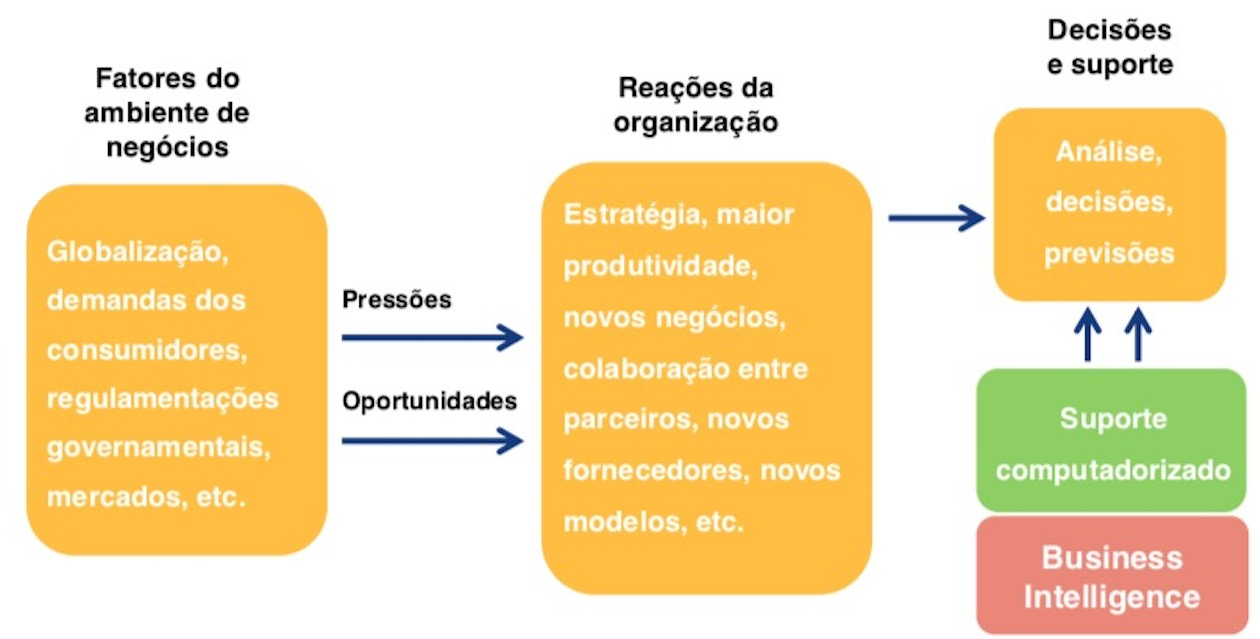
\includegraphics[width=0.6\textwidth]{./04-figuras/figura-01}
    \label{fig:ilustfig01}
\end{figure}
\vspace*{-0,9cm}
{\raggedright \fonte{Disponível em: <https://Portal (www.fp2.com.br)>. Acesso em: 10 ago. 2020.}}\\

\subsection{A arquitetura e componentes}

Como j\'{a} mencionado temos como base os estudos de Kimball (2013), seus elementos de arquitetura est\~{a}o representados na figura 2, como ilustrado, para Kimball (2013), existem quatro componentes separados e distintos a serem considerados no ambiente DW/BI: sistemas de origem operacional, sistema ETL, \'{a}rea de apresenta\c{c}\~{a}o de dados e aplicativos de inteligência de negócios.

\begin{figure}[H]
	\vspace*{0,2cm}
    \centering
    \caption{Elementos principais da arquitetura Kimball DW/BI.}
    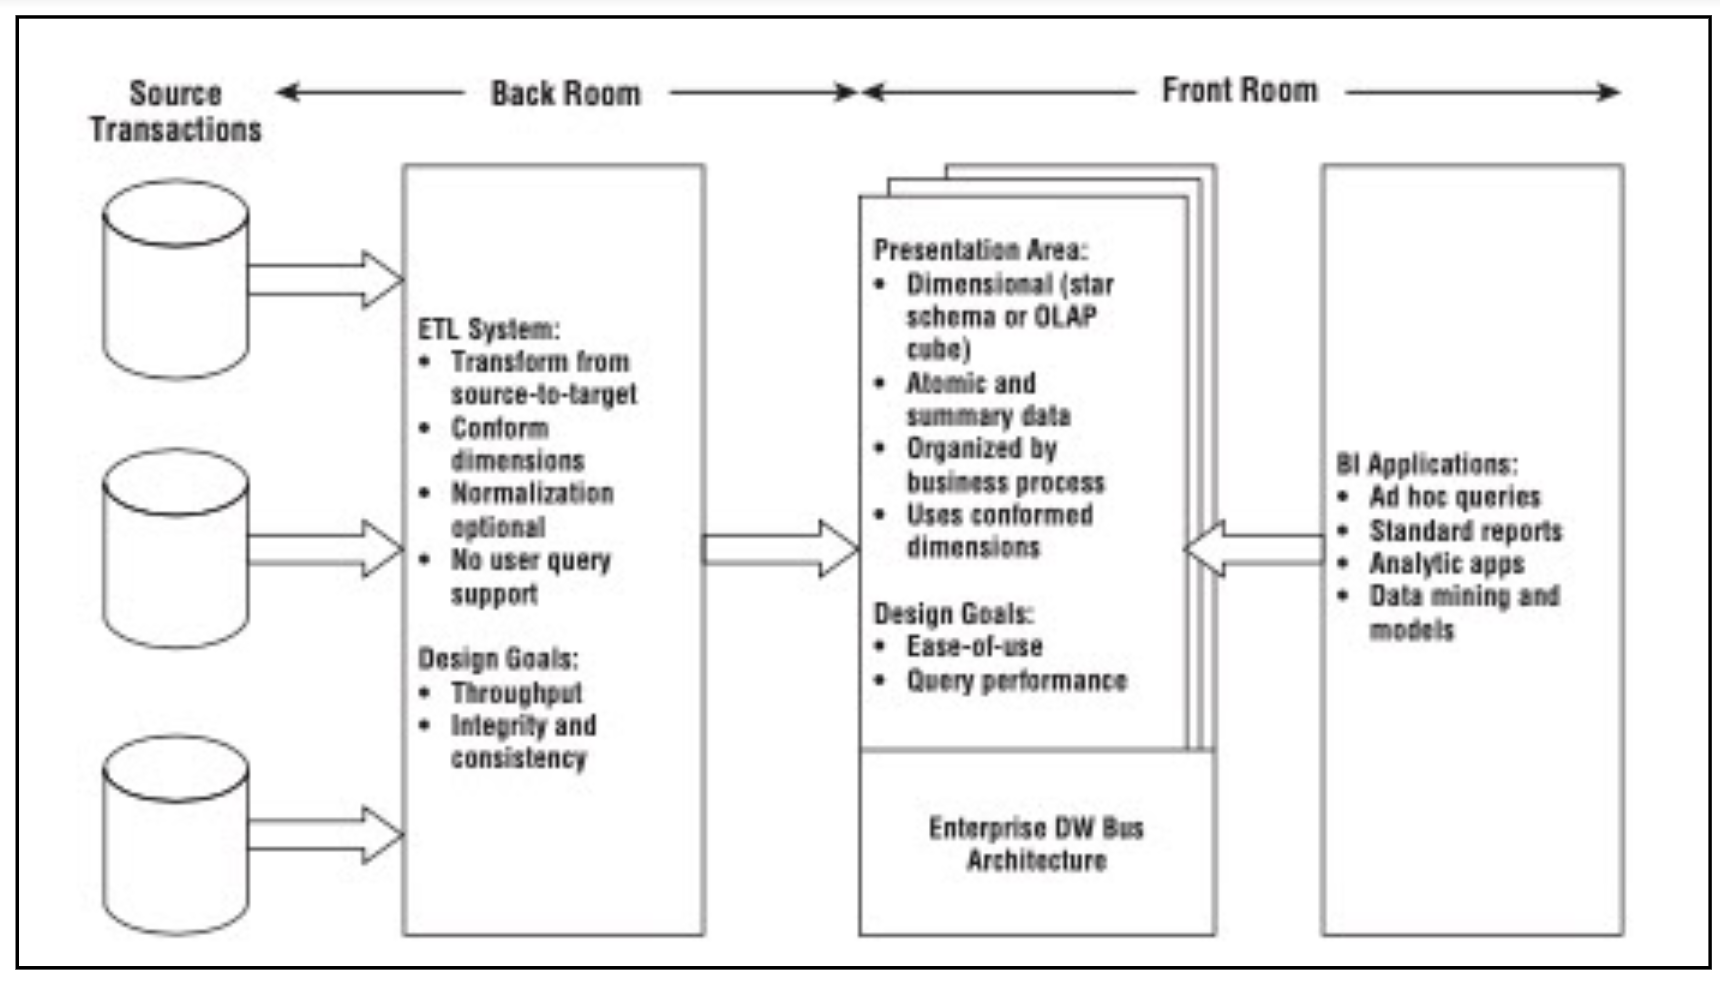
\includegraphics[width=0.6\textwidth]{./04-figuras/figura-02}
    \label{fig:ilustfig02}
\end{figure}
\vspace*{-0,9cm}
{\raggedright \fonte{ \textit{Core elements of the Kimball DW/BI architecture,  Kimball (2013)}}}\\


O primeiro dele \'{e} o \textit{Operational Source Systems} que s\~{a}o os sistemas operacionais de registro ou origem que capturam as transa\c{c}ões da empresa. Pense nos sistemas de origem como fora do \textit{Data Warehouse}, porque, presumivelmente você tem pouco ou nenhum controle sobre o conteúdo e o formato dos dados nesses sistemas operacionais. 

As principais prioridades dos sistemas de origem s\~{a}o o desempenho e a disponibilidade do processamento. As consultas operacionais em rela\c{c}\~{a}o aos sistemas de origem s\~{a}o consultas estreitas, um registro por vez, que fazem parte do fluxo normal da transa\c{c}\~{a}o e severamente restringidas em suas demandas no sistema operacional.

O segundo \'{e} o ETL (\textit{Extract, Transformation, and Load System}) s\~{a}o os sistemas respons\'{a}veis pela: extra\c{c}\~{a}o, transforma\c{c}\~{a}o e carregamento. E que consiste em uma \'{a}rea de trabalho, estruturas de dados instanciadas e um conjunto de processos.

A cria\c{c}\~{a}o de estruturas normalizadas para o ETL e estruturas dimensionais para apresenta\c{c}\~{a}o, significa que os dados s\~{a}o potencialmente extraídos, transformados e carregados duas vezes - uma vez no banco de dados normalizado e depois novamente quando você carrega o modelo dimensional. 

A terceira \'{e} \textit{Presentation Area to Support Business Intelligence} \'{e} nela onde os dados s\~{a}o organizados, armazenados e disponibilizados para consulta direta por usu\'{a}rios, redatores de relatórios e outros aplicativos de BI analíticos.

A quarta \'{e} o \textit{Business Intelligence Applications} que \'{e} o componente final da arquitetura Kimball DW/BI. \'{e} o aplicativo de \textit{Business Intelligence} (BI) composto de uma variedade de recursos fornecidos aos usu\'{a}rios de negócios para alavancar a \'{a}rea de apresenta\c{c}\~{a}o para tomada de decis\~{a}o analítica.

Um aplicativo de BI pode ser t\~{a}o simples quanto uma ferramenta de consulta \textit{ad hoc} ou t\~{a}o complexo quanto um aplicativo sofisticado de minera\c{c}\~{a}o ou modelagem de dados. 

As ferramentas de consulta \textit{ad-hoc}, por mais poderosas que sejam, podem ser entendidas e usadas efetivamente apenas por uma pequena porcentagem da popula\c{c}\~{a}o potencial de usu\'{a}rios de negócios de DW/BI. 

Alguns dos aplicativos mais sofisticados, como ferramentas de modelagem e previs\~{a}o, podem fazer \textit{upload} de resultados de volta para os sistemas operacionais de origem, sistema ETL ou \'{a}rea de apresenta\c{c}\~{a}o.

\subsection{Níveis organizacionais}

Por padr\~{a}o as organiza\c{c}ões adotam abordagem de BI que abrange os três níveis hier\'{a}rquicos da organiza\c{c}\~{a}o: estrat\'{e}gico, t\'{a}tico e operacional. O BI tradicional, tamb\'{e}m conhecido como BI 1.0, abrange apenas os níveis estrat\'{e}gico e  t\'{a}tico. Por\'{e}m, o uso de BI tamb\'{e}m pode ser usado no nível operacional (IMHOFF, 2006; AIRINEI & HOMOCIANU, 2009; BALTZAN & PHILLIPS, 2012; TURBAN & VOLONIMO, 2013).

Segundo TURBAN e VOLONIMO (2013) a alta competitividade \'{e} o principal fator que influencia empresas a adotarem BI no nível operacional.

Nesse nível de competi\c{c}\~{a}o tamb\'{e}m se busca melhorar decisões, como dar respostas mais r\'{a}pidas aos clientes. O Quadro 1, abaixo, apresenta um comparativo entre os tipos de BI. Na primeira coluna, \'{e}apresentada a caraterística a ser comparada. Na segunda, como essa característica \'{e}vista no BI estratégico. Na terceira, como \'{e}no BI tático. Por fim, na última, como \'{e}no BI operacional.

A principal diferença está na temporalidade dos dados e no foco de negócio. O BI operacional deve ser imediato ou no mesmo dia e objetiva auxiliar o controle das operações diárias (TURBAN & VOLONIMO, 2013). Mesmo  assim, \'{e}importante que os três tipos sejam orientados e alinhados aos objetivos da organização (BALTZAN; e PHILLIPS, 2012).

\begin{quadro}[H]
	\begin{center}
		\caption{Comparativo entre as Características do BI Operacional, T\'{a}tico e Estratégico..\label{qua:quadro-01}}
	    \begin{tabular}{ |p{3cm}|p{3cm}|p{3cm}|p{3cm}| }
			\hline
		    Caracter\'{i}sticas & 
            BI Operacional & 
            BI T\'{a}tico & 
            BI Estrat\'{e}gico \\
		    \hline
            Foco principal do neg\'{o}cio &
            Administrar operações do dia a dia &
            Analisar dados; entregar relatórios & 
            Atingir as metas empresariais e longo prazo \\
            \hline
            Principais usu\'{a}rios &
            Gerente de setor &
            Executivos, analistas, gerentes de setor &
            Executivos, analistas \\
            \hline
            M\'{e}tricas &
            Métricas são individualizadas 
            para que o gestor de cada linha
            possa obter insight sobre o
            desempenho de seus processos de negócio
            &
            Métricas são um mecanismo de \textit{feedback}
            para companhar e entender como a estratégia
            está progredindo e quais ajustes precisam ser planejada
            &
            Métricas são um mecanismo de \textit{feedback}
            para companhar e entender como a
            estratégia está progredindo e quais ajustes
            precisam ser planejados
            \\
            \hline
            Prazo &
            Imediatamente, dentro do dia &
            Diário, semanal, mensal&
            Mensal, trimestral, anual \\
            \hline
            Tipos de dados ou usos  &
            Em tempo real ou quase em tempo real  &
            Histórico, preditivo  &
            Histórico, preditivo \\
            \hline
    	\end{tabular}
	\end{center}
	\vspace*{-0,8cm}
	{\raggedright \fonte{Elaborado à partir de\cite{bi-turban-2013}}
\end{quadro}

\subsection{Next Generation Business Intelligence ou BI 2.0}

Pode-se dizer que a tecnologia de \testint{Business Intelligence} n\~{a}o dispõe de um conceito pr\'{e}-definido, ou seja, pode ser compreendida e explicada de diversas formas, o mesmo acontece com a Next Generation Business Intelligence, muito embora sejam utilizados conceitos bem parecidos na sua defini\c{c}\~{a}o. 

O BI da segunda gera\c{c}\~{a}o concentra-se mais no contexto de fluxos de dados e no conhecimento, e n\~{a}o apenas nas informa\c{c}ões como o BI de primeira gera\c{c}\~{a}o. Ou seja, o BI 2.0 \'{e} como uma extens\~{a}o da Web 2.0 no cen\'{a}rio empresarial, tornando-se uma oportunidade importante para o usu\'{a}rio e ampliando os conhecimentos sobre a camada de apresenta\c{c}\~{a}o, visualiza\c{c}\~{a}o de dados e informa\c{c}ões sobre a demanda. Dados estruturados e n\~{a}o estruturados, empresarial e público, que incluem novos relatórios de an\'{a}lise e intera\c{c}\~{a}o.

O principal benefício do \textit{Next Generation Business Intelligence} para uma organiza\c{c}\~{a}o \'{e} a capacidade de fornecer informa\c{c}ões precisas quando necess\'{a}rio, incluindo uma vis\~{a}o em tempo real do desempenho corporativo. Para permitir adaptar os modelos de negócios para o mundo de hoje em tempo real, aplica\c{c}ões de software s\~{a}o criadas agora utilizando ED \testint{(event-driven)}, ou seja, dirigido a eventos. 

Assim os dados se movem em tempo real sobre arquiteturas orientadas a servi\c{c}os, utilizando servi\c{c}os de baixo acoplamento e altamente interoper\'{a}veis, ou seja, operacional em servi\c{c}os de v\'{a}rias formas, que promovem a integra\c{c}\~{a}o de aplicativos padronizados.

Na Figura 3, os principais componentes de um sistema de \textit{Next Generation Business Intelligence} e uma breve explana\c{c}\~{a}o sobre cada um:

\begin{figure}[H]
	\vspace*{0,2cm}
    \centering
    \caption{Componentes de um sistema de BI 2.0.}
    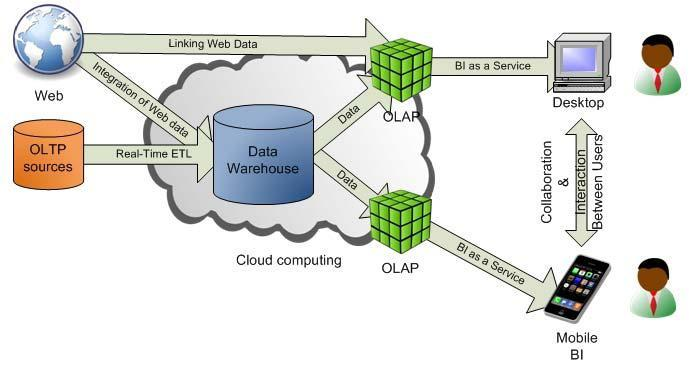
\includegraphics[width=0.6\textwidth]{./04-figuras/figura-03}
    \label{fig:ilustfig03}
\end{figure}
\vspace*{-0,9cm}
{\raggedright \fonte{Disponível em: Portal (www.devmedia.com.br), Processo de Cria\c{c}\~{a}o e Exposi\c{c}\~{a}o, disponível em: <https://www.devmedia.com.br/business-intelligence-2-0-conceitos-componentes-e-arquitetura/28899>, acessado em 5 jun de 2020.}}\\


Na figura acima nota-se que o BI 2.0 extrai dados n\~{a}o somente de um DW, mas sim de dados on-line e em tempo real com o auxílio do OLTP (On-line Transaction Processing) e do Real Time ETL (Processo ETL em tempo real). A seguir uma breve explica\c{c}\~{a}o sobre cada um de seus componentes. O bom est\'{a} ciente de que al\'{e}m das fontes de dados tradicionais, ou seja, transa\c{c}\~{a}o de dados, as fontes de dados de BI est\~{a}o evoluindo para incluir at\'{e} mesmo os mensagens enviadas por intranets empresariais e perfis pessoais de funcion\'{a}rios e clientes da web. Os dispositivos móveis e outros dados do sensor tamb\'{e}m s\~{a}o adicionados \`{a}s fontes de dados. Contudo, muitas dessas fontes de dados n\~{a}o s\~{a}o estruturadas. Para isto precisamos entender as tecnologias:

\begin{itemize}

    \item Web 2.0: Novas pr\'{a}ticas e abordagens da web com conteúdo dinâmicos e assíncronos\index{NewR}\footnote{Assíncronos: na \'{a}rea da tecnologia da informa\c{c}\~{a}o, a comunica\c{c}\~{a}o assíncrona \'{e} a transmiss\~{a}o de dados, geralmente sem o uso de um sinal de relógio externo, onde os dados podem ser transmitidos intermitentemente em um fluxo est\'{a}vel.} que possibilitam os usu\'{a}rios interagirem com a p\'{a}gina e com outros usu\'{a}rios, ex: Redes Sociais;
    \item OLTP (\textit{Online Transaction Processing}):, ou seja, processamento de transa\c{c}ões em tempo real. S\~{a}o sistemas que registram as transa\c{c}ões, como, por exemplo, os ERPs (\textit{Enterprise Resource Planning});
    \item \textit{Real Time ETL}: Processo de extra\c{c}\~{a}o, transforma\c{c}\~{a}o e carga de dados em tempo real. Basicamente falando \'{e} uma forma de integrar os dados em tempo real, podendo ser feitos por intervalos de lotes em curto espa\c{c}o de tempo ou dependendo do segmento feito apenas algumas vezes ao dia, ser\'{a} mais aprofundado no tópico 2.4;
    \item \textit{Data Warehouse}: Grande banco de dados ou armaz\'{e}m de dados, respons\'{a}vel pelo armazenamento de altos volumes de dados, ou seja, os dados brutos de uma organiza\c{c}\~{a}o, teremos no tópico 2.5, mais detalhes sobre DW; 
    \item \textit{Data Mart}: Repositório de dados, subdivis\~{a}o de um DW, tamb\'{e}m respons\'{a}vel pelo armazenamento de dados, por\'{e}m mais específicos e em menor escala, no tópico 2.6, daremos ênfase ao DM.
    \item OLAP: An\'{a}lise e processamento on-line de dados, conhecidos tamb\'{e}m como cubos decisórios, local onde os dados s\~{a}o analisados e processados gerando informa\c{c}ões essenciais ao negócio, tópico 2.8; 
    \item \textit{Cloud Computing}: Que se refere a computa\c{c}\~{a}o nas nuvens e tem como base a utiliza\c{c}\~{a}o da memória e das capacidades de armazenamento, compartilhados e interligados por meio da Internet;
    \item \textit{Linking Web Data}: Refere-se a dados ligados descrevendo um m\'{e}todo de publica\c{c}\~{a}o de dados estruturados que podem ser interligados baseando-se em tecnologias da web estendendo-se para compartilhar informa\c{c}ões que podem ser lidos automaticamente por computadores; 
    \item \textit{Integration of Web Data}: Refere-se \`{a} integra\c{c}\~{a}o de dados, essa integra\c{c}\~{a}o combina dados residentes em diferentes fontes, tendo em vista fornecer aos usu\'{a}rios uma vis\~{a}o única dos dados;
    \item \textit{BI as a Service}: Refere-se \`{a} arquitetura SOA\index{NewR}\footnote{SOA \textit{(Service-Oriented Architecture)}: Significa, Arquitetura Orientada a Servi\c{c}os, numa tradu\c{c}\~{a}o livre. O conceito foi proposto pela primeira vez em 1996, no artigo “Service Oriented Architectures” (abril de 1996), escrito pelos pesquisadores Roy Schulte e Yefim Natis do Gartner Group, e \'{e} um estilo de arquitetura de software cujo princípio fundamental prega que as funcionalidades implementadas pelas aplica\c{c}ões devem ser disponibilizadas na forma de servi\c{c}os.}, orientado a servi\c{c}os, o que facilita a partilha e acesso de informa\c{c}ões em tempo real.

\end{itemize}

A arquitetura orientada a servi\c{c}os (SOA) abriu caminho para o BI 2.0, pois facilita o acesso em tempo real e a coleta de dados. BI 2.0 \'{e} tamb\'{e}m mais uma vis\~{a}o de web orientada de dados tradicionais de consulta e ferramentas de an\'{a}lise.

A arquitetura de uma aplica\c{c}\~{a}o de BI 2.0 difere em alguns pontos da arquitetura de uma aplica\c{c}\~{a}o de BI tradicional ou BI 1.0. A base da arquitetura foi praticamente mantida, por\'{e}m alguns componentes foram inseridos, tais como: Web 2.0, \textit{Real Time ETL}, OLTP, Redes Sociais, Software como um servi\c{c}o.

Levando-se em considera\c{c}\~{a}o que o objetivo do BI 2.0 \'{e} reduzir a latência, ou seja, o tempo. Torna-se necess\'{a}rio reduzir o tempo entre quando um evento ocorre e quando uma a\c{c}\~{a}o \'{e} tomada, a fim de melhorar o desempenho empresarial, esse \'{e} o foco das arquiteturas de BI 2.0. A arquitetura BI 2.0 abrir\'{a} uma s\'{e}rie de op\c{c}ões para a criatividade dos usu\'{a}rios de negócios operacionais. 

Esta próxima gera\c{c}\~{a}o de BI 2.0 inclui recursos de visualiza\c{c}\~{a}o que permitem aos usu\'{a}rios ver as rela\c{c}ões entre os dados, interatividade que lhes permitem manipular os dados e uma forma intuitiva de trabalho que combina com o modo com que os usu\'{a}rios de negócios pensam, por exemplo, em fazer perguntas novas que podem surgir. 

Ferramentas de BI 2.0 s\~{a}o mais intuitivas para os usu\'{a}rios de negócios do que as ferramentas tradicionais de negócios, software de inteligência especial e planilhas.

Finalizando esta se\c{c}\~{a}o um breve comparativo do BI tradicional ou BI 1.0 com o BI 2.0, demonstra-se na quadro abaixo as principais características existentes entre eles.

\begin{quadro}[H]
	\begin{center}
		\caption{Comparativo: BI Tradicional verso BI 2.0.\label{qua:quadro-02}}
	    \begin{tabular}{ |p{7cm}|p{7cm}| }
			\hline
		    Características Tradicional ou BI 1.0  
		    & 
            \textit{Next Generation Business Intelligence} ou BI 2.0 
            \\
		    \hline
            Envio e apresentação de relatórios estáticos para os usuários. Relatórios orientados para impressão. Análise de relatório pós-fato devido à latência dos dados. 
            &
            Comunidades de usuários dinâmicos com colaboração ativa e compartilhamento imediato de informações, onde os usuários elaboram seus próprios relatórios. Aplicações de geração de relatórios interativos e baseados na Web 2.0. Relatórios em tempo real. 
            \\
            \hline
            Custo elevado é considerado um luxo dentro da organização. (Empresas de grande porte). 
            &
            Soluções econômicas e rentáveis disponibilizadas para as organizações como um todo. (Pequenas, Médias e Grandes empresas).
            \\
            \hline
            Gráficos com barras estáticas, e gráficos circulares segmentados. 
            &
            Visualização de dados intuitiva, dinâmica e interativa.
            \\
            \hline
            Modelo OLAP para análise. 
            &
            Modelo OLAP junto com outras alternativas inovadoras, menos complexas e de alto.
            \\
            \hline
            Instalação, upgrade e uso complexo e de alto consumo de tempo. 
            &
            Instalação, upgrade e uso simplificados.
            \\
            \hline
            Parâmetros de pesquisa predefinidos. 
            &
            Pesquisas dinâmicas ou de estilo livre permitindo a exploração de dados.
            \\
            \hline
            Dados estruturados. 
            &
            Conjunto ampliado de tipos de dados suportados, inclusive dados não estruturados e serviços XML da web.
            \\
            \hline
            Licenciamento de software por usuário. 
            &
            Licenciamento de software por servidor para um número ilimitado de usuários ou licenciamento baseado em assinatura..
            \\
            \hline
            BI para todos, na medida da necessidade da organização.
            \\
           \hline
	    \end{tabular}
	\end{center}
	\vspace*{-0,8cm}
	{\raggedright \fonte{Disponível em: <https://www.devmedia.com.br>. Acesso em: 12 ago. 2020.}}
\end{quadro}


Assim, com base na tabela 2, podemos dizer que o BI 2.0, apresenta inova\c{c}ões e novas pr\'{a}ticas que o torna mais eficaz em rela\c{c}\~{a}o ao BI tradicional, por\'{e}m aos poucos e na pr\'{a}tica, ele traz muitos questionamentos e dúvidas em rela\c{c}\~{a}o ao seu funcionamento e desempenho no dia-a-dia

\subsection{Tendências futuras}

Antes de concluirmos esta revis\~{a}o liter\'{a}ria, falaremos um poucos sobre as tendências para o futuro do Business Intelligence. Entre as principais est\~{a}o: an\'{a}lises preditivas e prescritivas, inteligência artificial, inteligência empresarial colaborativa, seguran\c{c}a das informa\c{c}ões, gest\~{a}o de pessoas, e o monitoramento da concorrência.

A An\'{a}lises Preditivas pode ser resumida como \`{a} pr\'{a}tica de extrair informa\c{c}ões relevantes pensando em prever futuras probabilidades. J\'{a} na an\'{a}lise prescritiva, a previs\~{a}o do futuro n\~{a}o \'{e} o suficiente, \'{e} preciso encontrar uma forma de construí-lo.

A Inteligência Artificial (AI), que para muitos ainda pare\c{c}a um tema de fic\c{c}\~{a}o científica, est\'{a} sendo bastante usada em diversos campos da TI, e vem forte para os próximos anos e ser\'{a} uma pe\c{c}a fundamental para o \textit{Business Intelligence}. O maior motivo para seu uso e a melhora de qualidade dos processos que envolvem as tomadas de decis\~{a}o das organiza\c{c}ões. Simples assim.

A Inteligência Empresarial Colaborativa, \'{e} est\'{a} em um contexto em que inúmeras empresas ao redor do mundo j\'{a} chegaram \`{a} conclus\~{a}o de que para aumentar as chances de sucesso do negócio, \'{e} necess\'{a}rio adotar uma gest\~{a}o colaborativa e que contribua para todos os colaboradores no que diz respeito \`{a} consecu\c{c}\~{a}o dos resultados.

A Gest\~{a}o de Pessoas, \'{e} outra tendência onde o BI pode ajudar a promover o conhecimento dos funcion\'{a}rios acerca dos seus processos. A ideia maior \'{e} tornar as equipes mais conscientes sobre os erros, objetivos e metas pontuais.

O monitoramento da concorrência, \'{e} indispens\'{a}vel para todo e qualquer tipo de organiza\c{c}\~{a}o que queira sair na frente e estar mais alinhada \`{a}s necessidades de seu  público alvo. Nesse ponto, o Business Intelligence \'{e} fator imprescindível para o entendimento dos concorrentes: isso inclui o que eles andam fazendo e o que os clientes est\~{a}o falando sobre eles.
Vale salientar que essas tendências, poder\~{a}o mudar com as inova\c{c}ões no mundo complexo da TI.

\subsection{Benefícios e aplica\c{c}ões}

De acordo com NORONHA (2013): “a grande vantagem do conceito de Business Intelligence \'{e}justamente a capacidade que o sistema possui para ‘traduzir’ os dados armazenados em uma linguagem de fácil assimilação pelo corpo gerencial das empresas. Esse ambiente gerencial geralmente \'{e}caracterizado por gráficos que permitem a rápida interpretação de uma situação”.

Logo os gestores poderão ter acesso às informações “rapidamente” e poderão abreviar o tempo de resposta melhorando assim os processos decisórios. Dessa forma, a informação será o verdadeiro capital integralizado da empresa trazendo conhecimento para as decisões imediatas e para aquelas que virão no futuro.

Abaixo as vantagens do uso e aplicação do BI nas organiza\c{c}ões:

\begin{itemize}

    \item Incorporar os projetos de tecnologia com as metas estabelecidas pelas empresas na busca do máximo retorno do investimento;
    \item Compreender as tendências dos negócios, melhorando a consistência no momento de decisão de estratégias e ações a serem tomadas;
    \item Facilitar a identificação de riscos;
    Planejamento corporativo mais amplo;
    \item Facilitar o acesso e distribuir informação de modo mais amplo para obter envolvimento de todos dentro da empresa;
    Oferecer dados estratégicos para análise com um mínimo de atraso em relação a uma transação ou evento dentro da empresa;
    \item Automatização da informação de mapas de indicadores, evitando procedimentos manuais e rotineiros, obtendo diminuição dos custos operacionais;
    \item Visualização dinâmica cruzada: apresentação disponibilizada em várias perspectivas;
    \item Importação direta de dados de outras aplicações (ex.: Excel, Sistemas Legados, Sistemas Satélites e outras bases de dados), para tratamento dessas informações;
    \item Passagem dos dados estáticos para informações dinâmicas;
    Permite maior flexibilidade das informações das diversas fontes;
    \item Utilização da aplicação por seleção das variáveis de análise (arrastamento e/ou filtragem por um valor determinado dessa variável);
    \item Informação sempre atualizada, mediante definição e parametrização prévia.
 
 \end{itemize}
 
\subsection{Ferramentas de BI}

O conjunto de soluções para BI multiplicou-se e a diversidade de produtos \'{e}muito grande e continua em constante evolução e crescimento tecnológico.

\'{e}possível encontrar desde pacotes pré-configuráveis, at\'{e}ferramentas “engessadas” e inclusive soluções que permitem às empresas se aventurarem no desenvolvimento de um sistema totalmente caseiro.
Estas ferramentas têm em comum a característica de facilitar a transformação dos “amontoados de dados” em informações de forma a auxiliar os diversos níveis de uma empresa na tomada segura de decisões.

A seguir são enumerados algumas ferramentas que auxiliam a implantar o conceito de BI:

\begin{itemize}
    \item Planilhas eletrônicas;
    \item Geradores de consultas baseadas em SQL;
    \item Sistemas de apoio à decisão (DSS);
    \item EIS;
    \item Linguagem MDX;
    \item Ferramentas OLAP;
    \item Ferramentas KDD;
    \item Ferramentas de BAM;
    \item Ferramentas ETLs;
    \item Ferramentas metadados;
    \item Ferramentas BPM;
    \item Ferramentas Data Mining.
\end{itemize}

\subsection{Construir e Implementar um BI}

Primeiramente deve-se identificar as reais necessidades da empresa, especialmente as das áreas de vendas e marketing e, posteriormente, das finanças. Ou, no caso da geração de indicadores de desempenho, todas as principais áreas da empresa. 

Também deve ficar claro que apesar desses projetos envolverem o uso das ferramentas e soluções de tecnologia da informação, \'{e}importante entender que BI \'{e}um projeto de negócios e por isso deve estar alinhado à estratégia global da corporaçã
.
Contudo, trabalhar o conhecimento usando o BI \'{e}uma linha tênue e precisa estar sempre bem “presa” às definições dos processos evolutivos da empresa, conforme a figura 4, que informa os cinco passo para a crian\c{c}\~{a}o de uma solu\c{c}\~{a}o de BI, em conjunto com novas práticas comerciais, em melhores maneiras de relacionamento com os clientes e em novas formas de sobrevivência visando sempre usar a inteligência na tomada de decisão precisa e coerente.

\begin{figure}[H]
	\vspace*{0,2cm}
    \centering
    \caption{Composição do BI em cinco passos.}
    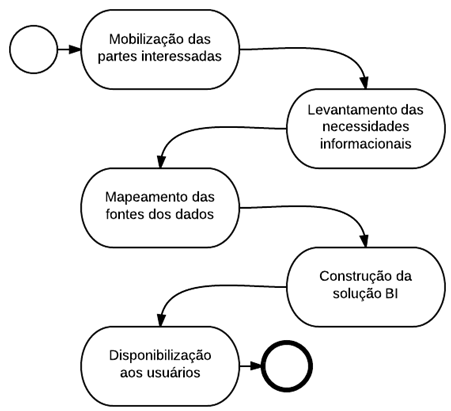
\includegraphics[width=0.6\textwidth]{./04-figuras/figura-04}
    \label{fig:ilustfig04}
\end{figure}
\vspace*{-0,9cm}
{\raggedright \fonte{Disponível em: <https://canaltech.com.br>. Acesso em: 11 ago. 2020.}}\\


Essas cinco etapas constituem uma vis\~{a}o geral de todo o processo necess\'{a}rio para a completa implementa\c{c}\~{a}o e implanta\c{c}\~{a}o de uma solu\c{c}\~{a}o de BI. Todavia, a qualidade final do projeto de BI vai depender muito da aten\c{c}\~{a}o dada a cada uma dessas atividades, que descreveremos abaixo:

\begin{itemize}

    \item Mobiliza\c{c}\~{a}o das partes interessadas: para início do projeto de BI, todos os \textit{stakeholders}\index{NewR}\footnote{Stakeholder: \'{e} um dos termos utilizados em diversas \'{a}reas como gest\~{a}o de projetos, comunica\c{c}\~{a}o social administra\c{c}\~{a}o e arquitetura de software referente \`{a}s partes interessadas que devem estar de acordo com as pr\'{a}ticas de governan\c{c}a corporativa executadas pela empresa.} devem ser mobilizados. Sem a participa\c{c}\~{a}o dos interessados, e principalmente do patrocínio da alta gest\~{a}o, o BI provavelmente fracassar\'{a};
    
    \item Levantamento das necessidades informacionais: na atividade de levantamento das necessidades procuramos entender quais as informa\c{c}ões exigidas pelos gestores. Nessa etapa estamos procurando listar todas as solicita\c{c}ões sem nos preocupar, neste momento, com a existência "real" dos dados;
    
    \item Mapeamento das fontes dos dados: o mapeamento da origem dos dados \'{e} feito após o levantamento das necessidades. Aqui \'{e} confrontando a viabilidade das solicita\c{c}ões efetuadas na etapa anterior. Caso afirmativo, s\~{a}o mapeadas as fontes dos dados para a posterior extra\c{c}\~{a}o na constru\c{c}\~{a}o do sistema de BI;
    
    \item Constru\c{c}\~{a}o da solu\c{c}\~{a}o BI: nessa etapa \'{e} iniciada a constru\c{c}\~{a}o propriamente dita da solu\c{c}\~{a}o. Se trata, sem dúvida alguma, da maior etapa do processo. Todas as atividades de extra\c{c}\~{a}o, qualidade dos dados, carga e teste das informa\c{c}ões s\~{a}o realizadas nesta etapa;
    
    \item Disponibiliza\c{c}\~{a}o aos usu\'{a}rios: depois de percorrido todas as etapas anteriores, chegamos, enfim \`{a} última etapa: disponibiliza\c{c}\~{a}o. Esta \'{e} uma etapa muito delicada, pois se trata do momento onde \'{e} entregue o produto de todo o esfor\c{c}o ao usu\'{a}rio final. Se a etapa de mobiliza\c{c}\~{a}o realizada no início do processo tiver êxito, dificilmente teremos problemas na disponibiliza\c{c}\~{a}o. Nesta etapa, al\'{e}m de entregar a solu\c{c}\~{a}o, ser\'{a} feito toda a capacita\c{c}\~{a}o aos gestores e analistas que utilizar\~{a}o a ferramenta no dia a dia para a consulta de informa\c{c}ões de apoio \`{a}s decisões.

\end{itemize}

Para construir um BI, primeiramente \'{e} feita a extra\c{c}\~{a}o e a an\'{a}lise dos dados da base ou das bases de dados, providos de uma gama de sistemas, os mesmos passam por um processo de transforma\c{c}\~{a}o (ETL).  

Faz-se uma limpeza deixando somente as informa\c{c}ões que ser\~{a}o úteis para a empresa. Após esse processo de transforma\c{c}\~{a}o \'{e} criado os \textit{Data Marts}, ambos definidos na fase de implementa\c{c}\~{a}o, onde \'{e} feita a organiza\c{c}\~{a}o de todas as informa\c{c}ões. 

Analisando e correlacionando os dados onde posteriormente ser\~{a}o passados por outro processo de transforma\c{c}\~{a}o preparando-os para serem armazenados em um repositório de dados denominado \textit{Data Warehouse}. 
Assim, quando os dados est\~{a}o no DW, todos organizados contendo somente as informa\c{c}ões relevante para o bom desenvolvimento da empresa \'{e} feita a explora\c{c}\~{a}o desses dados. 

Gerando informa\c{c}ões úteis para os usu\'{a}rios, sendo mostradas de diversas formas, atrav\'{e}s de gr\'{a}ficos, relatórios entre outros, esse processo \'{e} feito utilizando as ferramentas OLAP, que nos oferece uma interface interativa com o usu\'{a}rio.

\section{As Principais fontes de dados}

As Fonte de dados \'{e} o local onde s\~{a}o armazenados os dados que ser\~{a}o coletados por programas de computador \textit{(softwares)} para ent\~{a}o serem transformados nas informa\c{c}ões que ir\~{a}o ajudar uma determinada \'{a}rea ou algumas \'{a}reas de negócio da sua empresa.

Alguns exemplos para que você entenda o que s\~{a}o fontes de dados:

\begin{itemize}

    \item Planilhas Eletrônicas (Excel);
    \item Banco de Dados;
    \item Arquivo CSV;
    \item Arquivo XML;
    \item Arquivos JSON;
    \item Documentos de texto (Bloco de Notas, Word, etc);
    \item Sistemas ERP;
    \item Sistemas CRM;
    \item Sociais, entre outras.
    
\end{itemize}

Conhecer e entender o que \'{e} uma fonte de dados \'{e} o ponto chave de todo o processo de implanta\c{c}\~{a}o de um BI, pois, deve-se ter certeza absoluta que os dados l\'{a} armazenados s\~{a}o íntegros. N\~{a}o existe limite para fonte de dados, obviamente que quanto mais fontes (confi\'{a}veis) mais informa\c{c}ões e conhecimentos ser\~{a}o geradas, consequentemente mais detalhes do seu negócio você ter\'{a}. Nada adianta você ter 10 (dez) fontes de dados que n\~{a}o se pode confiar. 

\'{e} melhor você ter 2 (duas) fontes de dados com total certeza da integridade do que 10 (dez) em situa\c{c}\~{a}o duvidosa. As fontes de dados s\~{a}o a base do BI, pois s\~{a}o esses os dados que ser\~{a}o coletados e transformados em informa\c{c}ões que por sua vez ir\~{a}o gerar previsões, an\'{a}lises, gr\'{a}ficos e relatórios que ser\~{a}o a fonte de \textit{insights}\index{NewR}\footnote{\textit{Insight}: \'{e} o entendimento de uma causa e efeito específicos dentro de um contexto específico. O termo insight pode ter v\'{a}rios significados relacionados: um peda\c{c}o de informa\c{c}\~{a}o o ato ou resultado de entender a natureza interior das coisas ou de ver intuitivamente uma introspec\c{c}\~{a}o um peda\c{c}o de informa\c{c}\~{a}o; o ato ou resultado de entender a natureza interior das coisas ou de ver intuitivamente (chamado noesis em grego) uma introspec\c{c}\~{a}o; o poder da observa\c{c}\~{a}o e dedu\c{c}\~{a}o aguda , discernimento e percep\c{c}\~{a}o, chamado intelec\c{c}\~{a}o ou um entendimento de causa e efeito com base na identifica\c{c}\~{a}o de relacionamentos e comportamentos em um modelo, contexto ou cen\'{a}rio.} e a base para a tomada de decisões de todos os colaboradores da organiza\c{c}\~{a}o.

\section{ETL (Extra\c{c}\~{a}o, Transforma\c{c}\~{a}o e Carga)}

Para Kimball (2013) o sistema de extra\c{c}\~{a}o, transforma\c{c}\~{a}o e carga (ETL) do ambiente DW/BI consiste em uma \'{a}rea de trabalho, estruturas de dados instanciadas e um conjunto de processos.

A extra\c{c}\~{a}o \'{e} a primeira etapa do processo de inser\c{c}\~{a}o de dados no ambiente de armaz\'{e}m de dados. Extrair significa ler e entender os dados de origem e copiar os dados necess\'{a}rios no sistema ETL para manipula\c{c}\~{a}o adicional. Neste ponto, os dados pertencem ao armaz\'{e}m de dados.

Depois que os dados s\~{a}o extraídos para o sistema ETL, existem inúmeras transforma\c{c}ões em potencial, como limpeza dos dados (corre\c{c}\~{a}o de erros de ortografia, resolu\c{c}\~{a}o de conflitos de domínio, tratamento de elementos ausentes ou an\'{a}lise em formatos padr\~{a}o), combina\c{c}\~{a}o de dados de v\'{a}rias fontes e desduplicar dados. 

A etapa final do processo ETL \'{e} a estrutura\c{c}\~{a}o física e o carregamento de dados nos modelos dimensionais alvo da \'{a}rea de apresenta\c{c}\~{a}o. Como a principal miss\~{a}o do sistema ETL \'{e} entregar as tabelas de dimensões e fatos na etapa de entrega, esses subsistemas s\~{a}o críticos.

Por outro lado, as tabelas de fatos s\~{a}o geralmente grandes e demoram para carregar, mas prepar\'{a}-las para a \'{a}rea de apresenta\c{c}\~{a}o \'{e} geralmente simples. 
Quando as tabelas de dimensões e fatos em um modelo dimensional s\~{a}o atualizadas, indexadas, fornecidas com agregados apropriados e com garantia de qualidade adicional, a comunidade de negócios \'{e} notificada de que os novos dados foram publicados.

Após validar os dados para conformidade com as regras de negócios definidas um-para-um e muitos-para-um, pode ser inútil dar o passo final da cria\c{c}\~{a}o de um banco de dados físico 3NF \textit{(Third Normal Form)}\index{NewR}\footnote{3NF (\textit{Third Normal Form} ou Terceira Forma Normal): \'{e} uma forma normal usada para normalizar um design de banco de dados para reduzir a duplica\c{c}\~{a}o de dados e garantir a integridade referencial, garantindo que: a entidade est\'{a} na segunda forma normal; Nenhum atributo n\~{a}o prim\'{a}rio (sem chave) depende transitivamente de qualquer chave, ou seja, nenhum atributo n\~{a}o prim\'{a}rio depende de outros atributos n\~{a}o primos. Todos os atributos n\~{a}o primos devem depender apenas das chaves candidatas.}, pouco antes de transformar os dados novamente em estruturas desnormalizadas para a \'{a}rea de apresenta\c{c}\~{a}o de BI.

Infelizmente, algumas iniciativas de DW/BI falharam miseravelmente, porque concentraram toda a sua energia e recursos na constru\c{c}\~{a}o de estruturas normalizadas, em vez de alocar tempo para o desenvolvimento de uma \'{a}rea de apresenta\c{c}\~{a}o dimensional que ofere\c{c}a suporte \`{a} melhor tomada de decisões de negócios. 

Segundo Kimball (2013), \'{e} aceit\'{a}vel criar um banco de dados normalizado para suportar os processos ETL; no entanto, esse n\~{a}o \'{e} o objetivo final. As estruturas normalizadas devem estar fora dos limites das consultas do usu\'{a}rio, pois elas derrotam os objetivos gêmeos de compreensibilidade e desempenho. 
Em resumo a ETL \'{e} a responsável pela preparação dos dados que farão parte
do \textit{Data Warehouse} ou \textit{Data Mart}. Ela se dá basicamente em três passos: extração, transformação e carga de dados.

\begin{figure}[H]
	\vspace*{0,2cm}
    \centering
    \caption{ciclo de vida do ETL em todo seu processo.}
    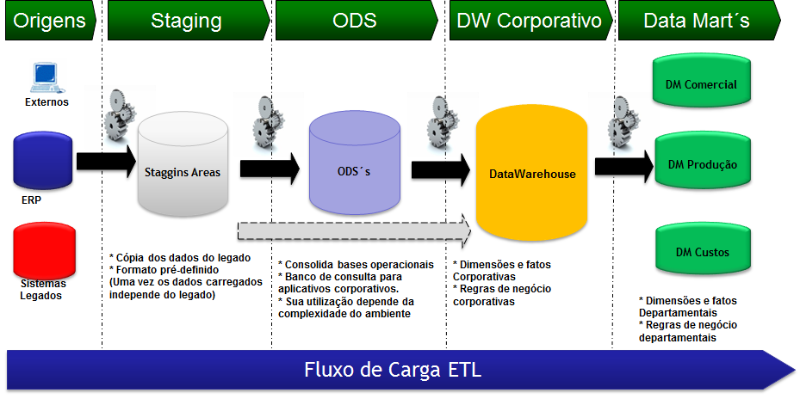
\includegraphics[width=0.6\textwidth]{./04-figuras/figura-05}
    \label{fig:ilustfig05}
\end{figure}
\vspace*{-0,9cm}
{\raggedright \fonte{Disponível em: <https://https://www.igti.com.br>. Acesso em: 13 ago. 2020.}}\\

\section{\textit{Data Warehouse}}

O \textit{Data Warehouse} conforme Inmon e Hackathorn (1997) \'{e}o ponto central da arquitetura de processamento de informações para sistemas de apoio á decisão (SAD), visto que suportam o processamento informacional através de um alicerce sólido de integração de dados corporativos e históricos para a realização de análises gerenciais.

De acordo com Kimball (2013), um bom DW pode aliviar os sistemas de origem de grande parte da responsabilidade de representar o passado.

Segundo Inmon (1997), \textit{Data Warehouse} pode ser definido como uma coleção de dados orientados a assuntos, sendo eles integrados, não voláteis e variáveis em relação ao tempo para apoio ao processo gerencial de tomada de decisão.

Esta definição acadêmica trás características importantes de um DW, que são melhor analisadas nas próximas sessões.

\subsection{Características}

Nas seguintes sessões são apresentadas características de suma importância para um \textit{Data Warehouse}.

\subsubsection{Orientação por assuntos}

A primeira característica notável do DW \'{e}a orientada por assunto, pois conforme Machado (2000), ela significa que o DW armazena as informações agrupadas por assuntos de interesse da empresa que são de maior importância.

Também cabe salientar que segundo Machado (2000), os projetistas de DW devem ter seu foco na modelagem dos dados e no projeto de banco de dados. Sendo que em um DW somente importam os dados que sejam importantes para a tomada decisão.

\subsubsection{Variação tempoos}

Conforme Inmon e Hackathorn (1997), todos os dados no DW são precisos em algum instante no tempo. Esta característica básica dos dados do DW \'{e}muito diferente das encontradas em um ambiente operacional, pois nela quando se acessa uma unidade de dados, \'{e}esperado que esta reflita valores corretos no momento do acesso.

Em virtude de os dados no DW serem corretos como em algum momento no tempo, conforme Inmon e Hackathorn (1997) são ditos que estes variam com o tempo.

A variação do tempo dos dados do DW segundo Inmon e Hackathorn (1997) apresentam-se de diversas maneiras. Conforme Machado (2000), a primeira e a mais simples \'{e}aquela que os dados representam informações sobre espaços de tempos de cinco a dez anos.

Já a segunda maneira são as estruturas básicas, onde cada estrutura contém um elemento tempo. E por fim a terceira maneira em que apresenta-se são os dados do DW, que uma vez armazenados corretamente, não podem ser atualizados (INMON; HACKATHORN, 1997).

\subsubsection{Não volatibilidadeos}

Conforme Inmon e Hackathorn (1997), outra característica definidora do DW trata-se do mesmo não ser volátil. A manipulação básica dos dados em um DW \'{e}muito mais simples do que em ambientes operacionais, pois de acordo com Machado (2000) existem apenas dois tipos de operações que podem ocorrer em um DW, a carga inicial do dados e o acesso em modo de leitura

\subsubsection{Integraçãoos}

Segundo Machado (2000), esta \'{e}uma das características de suma importância em um DW, pois todos os seus dados possuem um alto nível de integração.
Conforme Inmon e Hackathorn (1997), os dados ao serem movidos de um ambiente operacional orientado a aplicações para o DW, são integrados antes de serem incluídos no DW. Estes mesmos autores afirmam também que os dados precisam ser armazenados no DW de uma forma única, mesmo quando as aplicações armazenam os dados de modo diferente.

\subsection{Granularidade de dados}

Conforme Inmon (1997), o aspecto mais importante do projeto de um \textit{Data Warehouse} faz referência a questão da granularidade, pois diz respeito ao nível de detalhe ou de resumo contido nas unidades de dados existentes no DW. Segundo Machado (2000), quanto mais detalhe, mais baixo o nível de granularidade, quanto menos detalhe, mais alto o nível de granularidade.

O motivo no qual torna a granularidade a principal questão do projeto, de acordo com Inmon (1997) está no fato de que ela afeta profundamente o volume de dados que encontra-se no DW e, ao mesmo tempo, afeta o tipo de consulta que pode ser atendida.

Segundo Inmon (1997), o nível de granularidade exerce um profundo efeito tanto sobre as perguntas que podem ser respondidas, bem como sobre os recursos necessários para responder a uma pergunta.

A escolha do nível ou níveis de granularidade a serem utilizados em um projeto \'{e}indispensável para o sucesso. O método mais indicado para definir os níveis de granularidade conforme Machado (2000) está na utilização do bom senso e da análise detalhada das necessidades de informações levantadas para o projeto.
	
\subsection{Modelagem multidimensional}

Esta sessão tem como objetivo apresentar conceitos e terminologias empregadas no processo de modelagem e na sequência deste trabalho. 

\subsubsection{Dimensões}

Quando trata-se de dimensão, está se referindo aos elementos que participam de um fato, assunto de negócio. As dimensões determinam o contexto de um assunto de negócios (MACHADO, 2000).

As tabelas dimensionais conforme Kimball (1998), normalmente não possuem atributos numéricos, uma vez que são somente textuais e classificatórias dos elementos que participam de um fato.

Uma dimensão de acordo com Machado (2000) pode conter membros e hierarquias. Os membros são uma classificação de dados dentro de uma dimensão. Estes membros de uma dimensão podem ser arranjados em uma ou mais hierarquias, que por sua vez podem conter vários níveis hierárquicos.

\subsubsection{Fatos}

Segundo Kimball (2013), a tabela de fatos em um modelo dimensional armazena as medidas de desempenho resultantes dos eventos do processo de negócios de uma organiza\c{c}\~{a}o.
O termo fato representa uma medida de negócios. Imagine estar no mercado observando os produtos sendo vendidos e anotando a quantidade de unidades e a quantidade de vendas em dólar de cada produto em cada transa\c{c}\~{a}o de venda. Essas medidas s\~{a}o capturadas conforme os produtos s\~{a}o digitalizados no registro, conforme ilustrado na figura 6.

\begin{figure}[H]
	\vspace*{0,2cm}
    \centering
    \caption{Eventos de medi\c{c}\~{a}o de processo de negócios se traduzem em tabela de fato}
    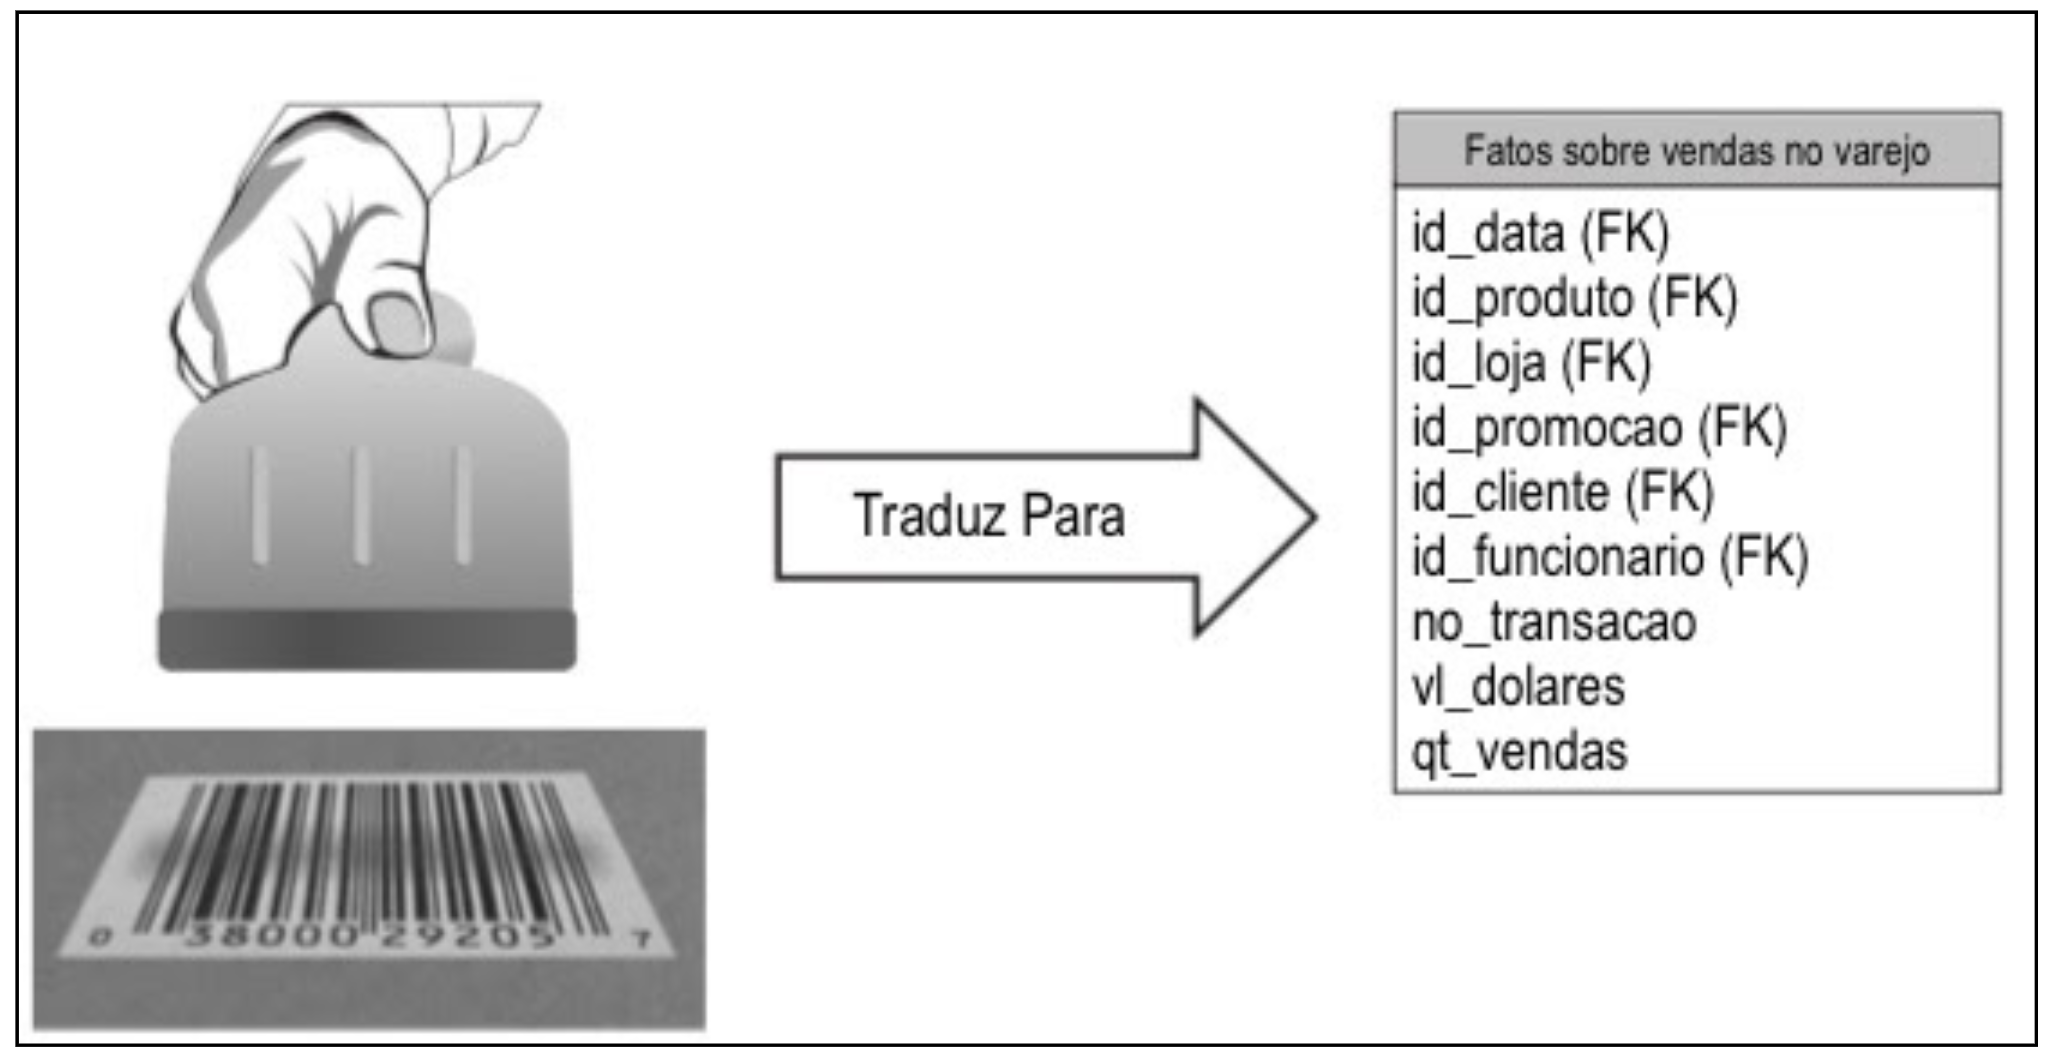
\includegraphics[width=0.6\textwidth]{./04-figuras/figura-06}
    \label{fig:ilustfig06}
\end{figure}
\vspace*{-0,9cm}
{\raggedright \fonte{adaptado de Kimball (2013)}}\\

Machado (2000), conceitua que um fato trata-se de uma coleção de itens de dados, composta de dados de medidas e de contexto. Um fato consiste em um item de negócio, uma transação de negócio ou um evento de negócio, nos quais se respondem as perguntas conforme figura 7. O mesmo \'{e}utilizado para verificar o processo de negócio de uma empresa.

De acordo com Kimball (1998), tudo aquilo que reflete a evolução dos negócios do dia-a-dia de uma instituição, \'{e}um fato.

\begin{figure}[H]
	\vspace*{0,2cm}
    \centering
    \caption{Fato}
    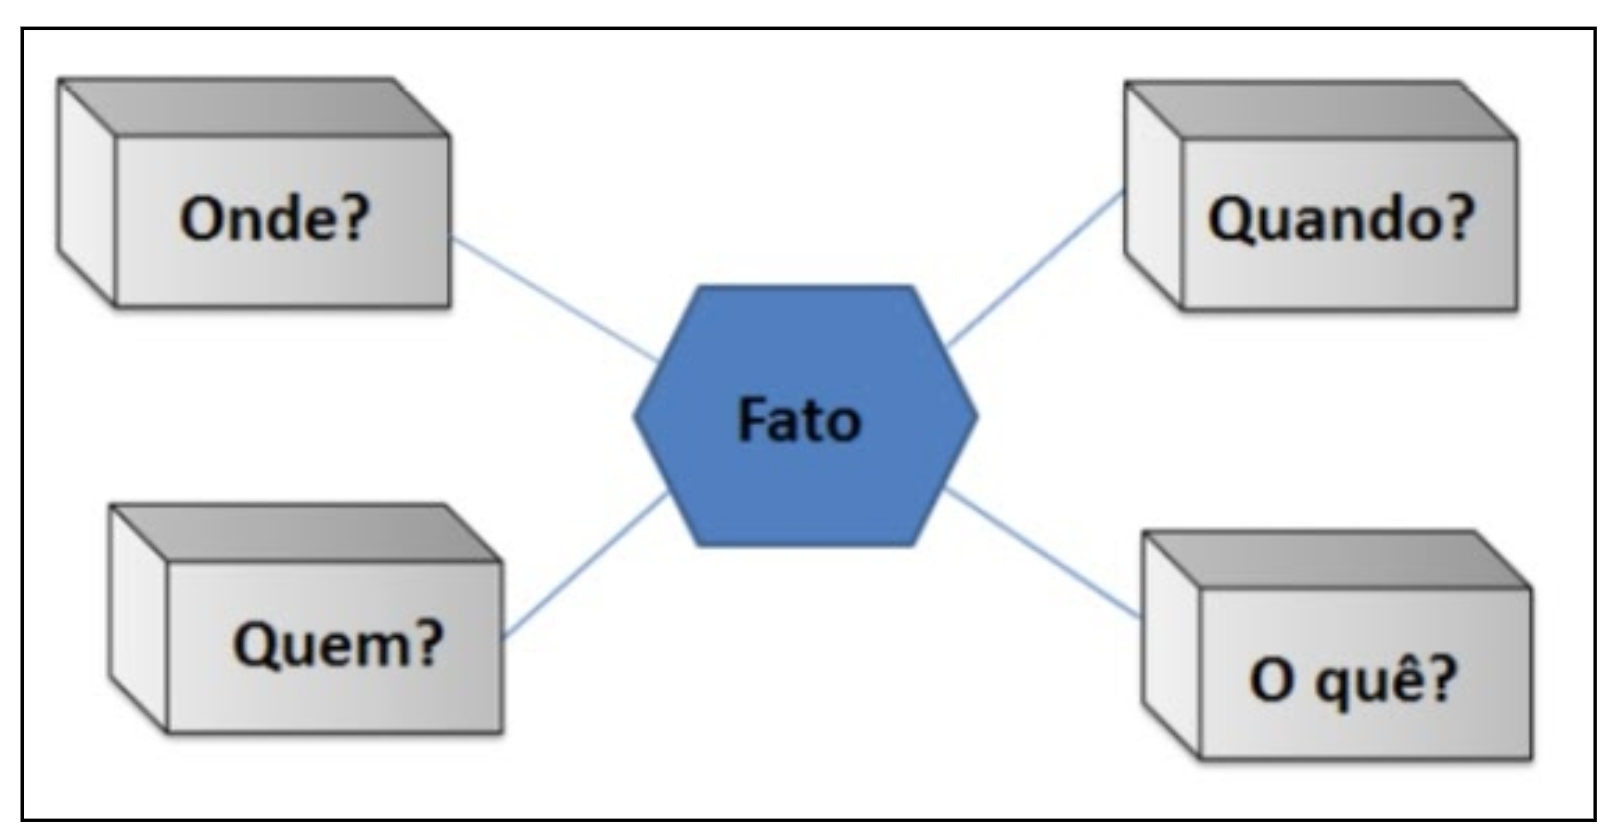
\includegraphics[width=0.6\textwidth]{./04-figuras/figura-07}
    \label{fig:ilustfig07}
\end{figure}
\vspace*{-0,9cm}
{\raggedright \fonte{adaptado de Machado (2000)}} \\

\subsubsection{Vari\'{a}veis}

As variáveis ou medidas são os atributos numéricos de um fato. Elas representam o desempenho de um indicador de negócios referente às dimensões que participam desse fato. Uma medida \'{e}estabelecida pela combinação das dimensões que pertencem a um fato (MACHADO, 2000).

\subsubsection{Opera\c{c}ões b\'{a}sicas}

Em um modelo de dados multidimensional se possuí operações básicas de 
OLAP \textint{(On- Line Analytic Processing)}.

Conforme Kimball (1998), OLAP \'{e}um termo inventado para descrever uma abordagem dimensional para o suporte à decisão.

Estas operações são usadas para analisar dados, sendo duas delas
:\textit{drill dow} e \textit{roll up}. Para poder-se utilizar estas operações devesse fazer valer da granularidade (MACHADO, 2000).

Com a capacidade do \textit{drill down} se esta diminuindo o nível da granularidade, aumentando assim o nível de detalhes. De maneira oposta a isso, 
o \textit{roll up} aumenta o nível da granularidade, diminuindo desta maneira, o nível de detalhes das informações.

\begin{figure}[H]
	\vspace*{0,2cm}
    \centering
    \caption{\textit{Drill Down} x  \textit{Roll Up}}
    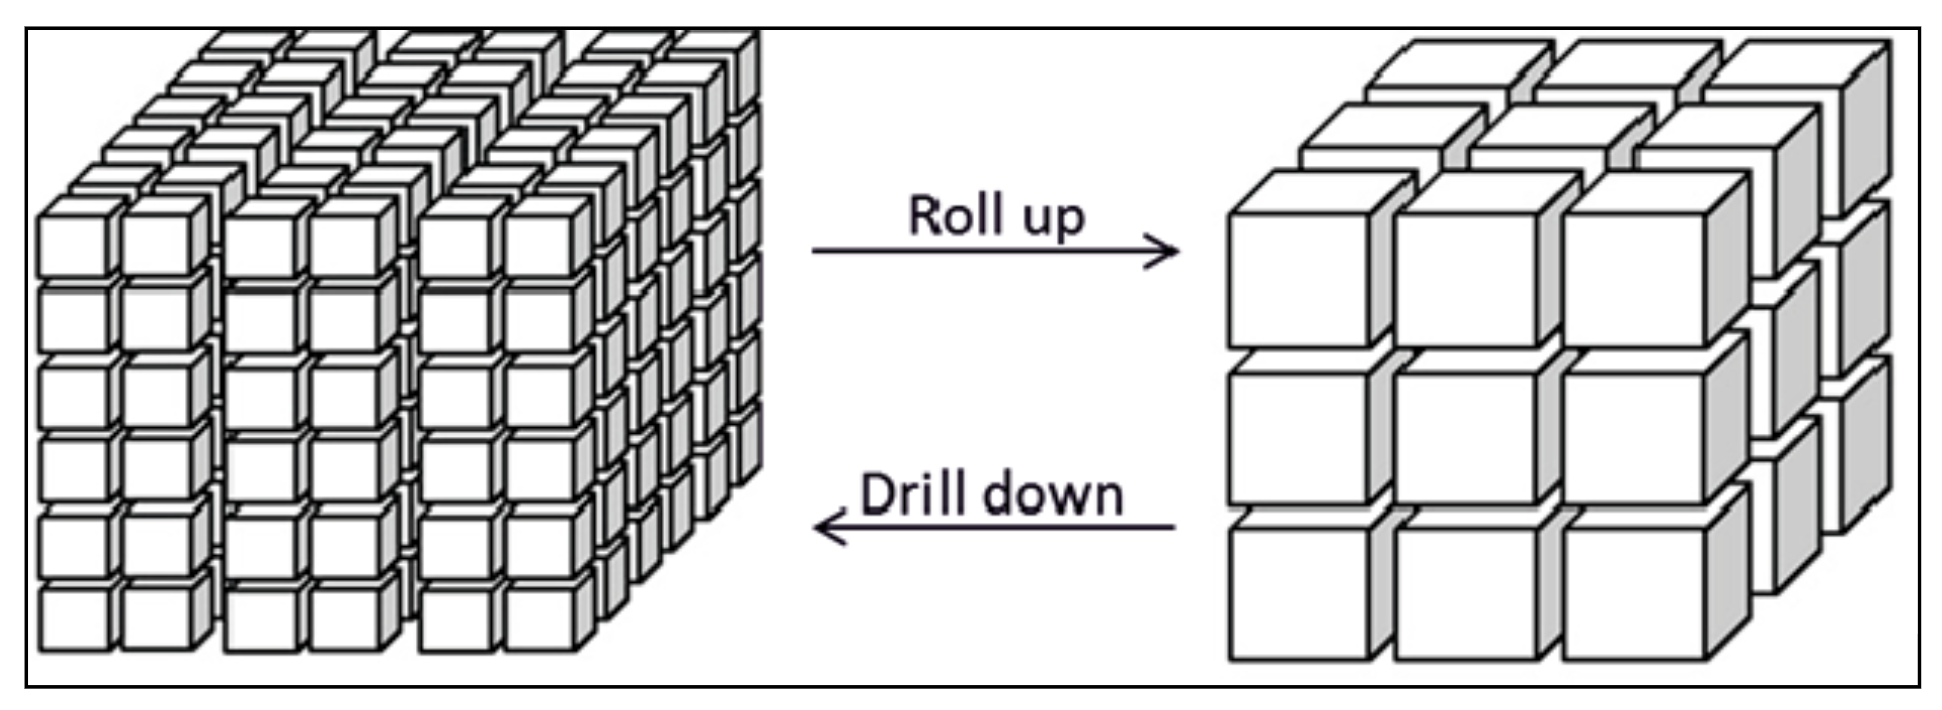
\includegraphics[width=0.6\textwidth]{./04-figuras/figura-08}
    \label{fig:ilustfig08}
\end{figure}
\vspace*{-0,9cm}
{\raggedright \fonte{Disponível em: <https://(https://www.researchgate.net/figure/
Roll-up-and-Drill-down-operations-fig3-282320388>. Acesso em: 12 ago. 2020.}}\\

Portanto conforme Machado (2000), estas operações permitem movimentar nossa visão dos dados ao longo dos níveis hierárquicos de uma dimensão.

\subsubsection{Modelo \textit{Star} (estrela)}

Em um modelo de dados multidimensional, a configuração que regula a organização dos fatos e das dimensões para armazenamento corresponde geralmente, a um esquema em estrela (MACHADO, 2000).

Este \'{e}composto por uma grande entidade central denominada tabela de fatos, e um conjunto de entidades menores denominadas tabelas de dimensões, que por sua vez estão organizadas ao redor da entidade central, formando assim uma estrela, conforme mostra a figura 9.

\begin{figure}[H]
	\vspace*{0,2cm}
    \centering
    \caption{Modelo Estrela}
    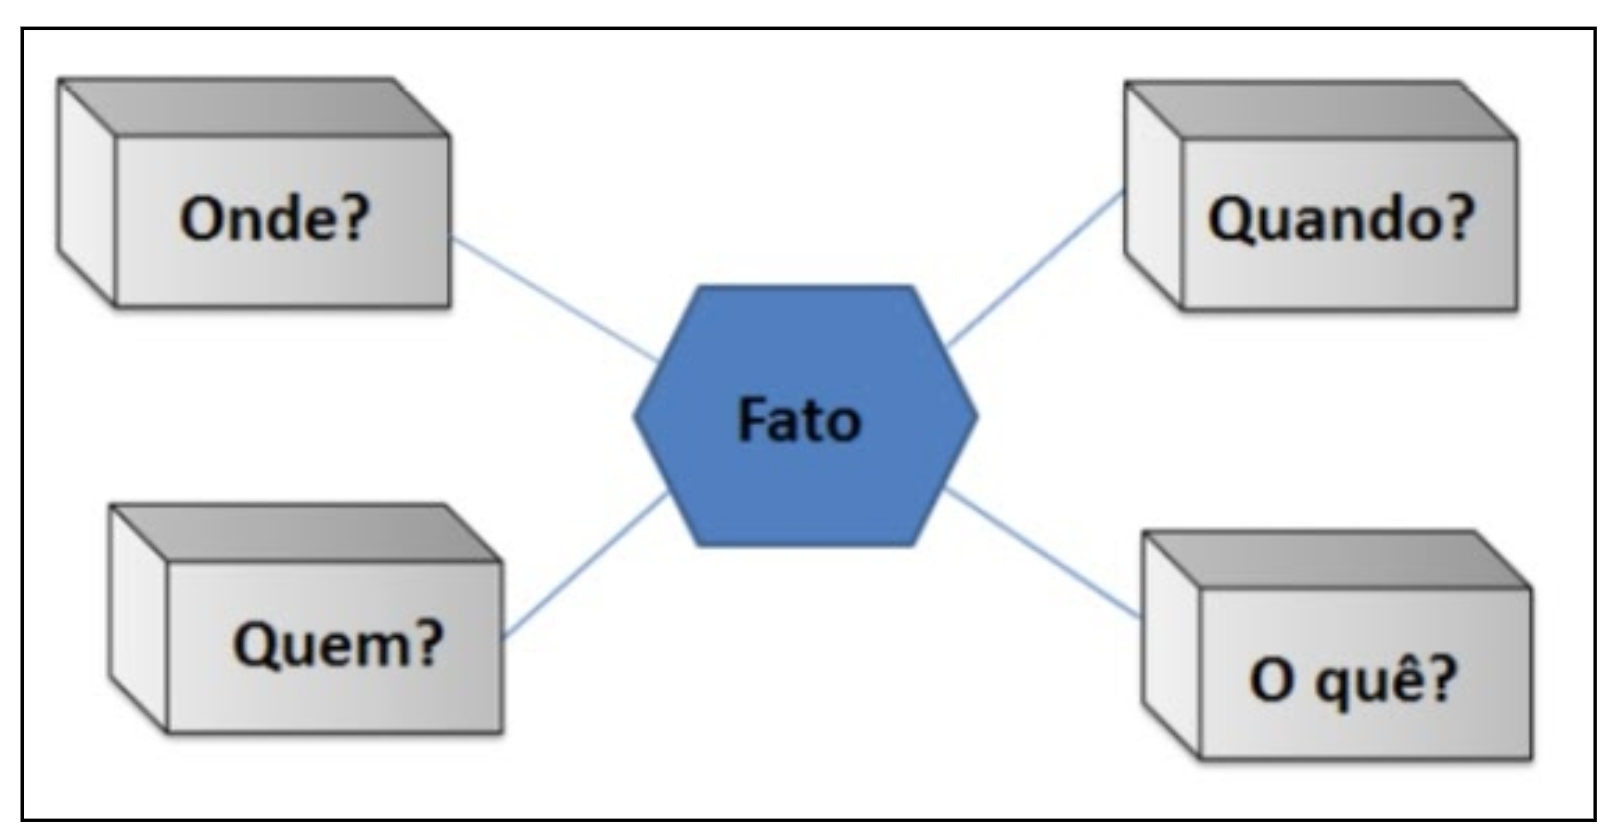
\includegraphics[width=0.6\textwidth]{./04-figuras/figura-09}
    \label{fig:ilustfig09}
\end{figure}
\vspace*{-0,9cm}
{\raggedright \fonte{adaptado de Machado (2000))}} \\

\subsubsection{Modelo \textit{Snowflake} (Floco de Neve)}

O modelo floco de neve da mesma forma que o modelo estrela possui uma entidade central denominada de fatos e um conjunto de entidades dimensão ao seu redor formando uma estrela
.
No entanto o modelo floco de neve de acordo com Machado (2000), \'{e}o resultado da decomposição de uma ou mais dimensões que possuem hierarquias entre seus membros. Conforme ilustrado na figura 10.
	
\begin{figure}[H]
	\vspace*{0,2cm}
    \centering
    \caption{Modelo Estrela}
    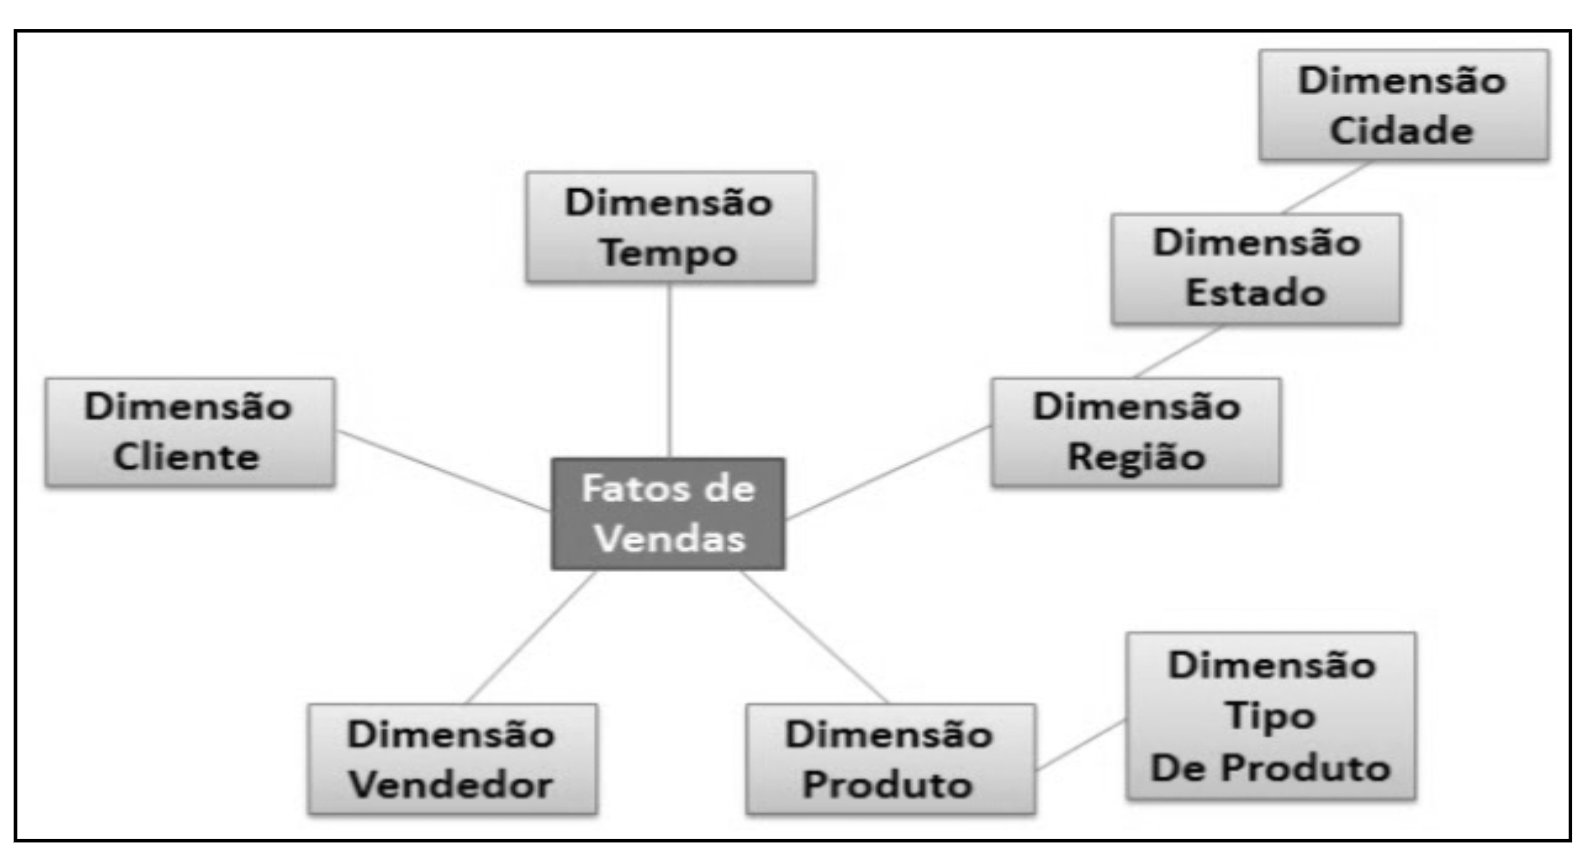
\includegraphics[width=0.6\textwidth]{./04-figuras/figura-10}
    \label{fig:ilustfig10}
\end{figure}
\vspace*{-0,9cm}
{\raggedright \fonte{adaptado de Machado (2000)}} \\

No entanto, conforme Machado (2000), um DW não possui inclusão de dados por meio de digitação, não necessitando assim garantir que os valores textuais sejam únicos, e nem tão pouco se preocupar com a economia de espaço, mas sim garantir o preceito de informação rápida.

O modelo floco de neve \'{e}esteticamente melhor para visualização de hierarquias, no entanto para se realizar consultas neste modelo são necessários mais joins, resultando assim em um gasto maior de tempo.
	
\section{\textit{Data Mart}}

Para Inmon (1997), um \textit{Data Mart} pode ser definido como um SGBD multidimensional que fornece uma estrutura bastante flexível de acesso a dados. Enquanto o DW extrai, transforma e limpa os dados dos sistemas transacionais, mantendo-os integrados em quantidades massivas e em seu nível mais baixo, o DM se serve destes dados, extraindo dados para um departamento ou uma área de negócio, oferecendo flexibilidade e controle ao usuário final, pois com o DM \'{e}possível fatiar e agrupar dados de diversas maneiras.

Para Machado (2000) e Kimball (1998b), os dados do \textit{Data Mart} são direcionados a um departamento ou a uma área específica do negócio e representam um subconjunto do DW corporativo.

O DM muitas vezes \'{e}visto como uma alternativa ao DW, pois custa menos e leva menos tempo para ser projetado e implementado. \'{e}criado para um grupo dirigido de usuários, normalmente um setor da empresa.

\section{KDD}

Extra\c{c}\~{a}o de conhecimento (tamb\'{e}m conhecido como processo KDD, do inglês 
\textit{(Knowledge Discovery in Databases)} \'{e} um processo de extra\c{c}\~{a}o de informa\c{c}ões de base de dados, que cria rela\c{c}ões de interesse que n\~{a}o s\~{a}o observadas pelo especialista no assunto, bem como auxilia a valida\c{c}\~{a}o de conhecimento extraído.

Assim, segundo FAYYAD, o KDD (Knowledge Discovery in Databases ou Descoberta do conhecimento em Banco de Dados) \'{e} uma tentativa de solucionar o problema causado pela "era da informa\c{c}\~{a}o": sobre carga de dados.

Por\'{e}m, a difini\c{c}\~{a}o mais conhecida eo KDD, diz que ele \'{e}o processo, não trivial, de extração de informações implícitas, previamente desconhecidas e potencialmente úteis, a partir dos dados armazenados em um banco de dados (FAYYAD et al., 1996)
O processo \'{e} n\~{a}o trivial , segundo FAYYAD (et al., 1996) j\'{a} que alguma t\'{e}cnica de busca ou inferência \'{e} envolvida, ou seja, n\~{a}o \'{e} apenas um processo de computa\c{c}\~{a}o direta. Os padrões descobertos devem ser v\'{a}lidos com algum grau de certeza, novos (para o sistema e de preferência tamb\'{e}m para o usu\'{a}rio), potencialmente úteis (trazer algum benefício) e compreensíveis (se n\~{a}o imediatamente ent\~{a}o depois da interpreta\c{c}\~{a}o).

O processo de busca de conhecimento cont\'{e}m uma s\'{e}rie de passos: sele\c{c}\~{a}o, pr\'{e}-processamento e limpeza, transforma\c{c}\~{a}o, minera\c{c}\~{a}o de dados (data mining) e interpreta\c{c}\~{a}o/avalia\c{c}\~{a}o. 
Simplificando, pode-se dizer que o processo de KDD compreende, na verdade, todo o ciclo que o dado percorre at\'{e} se transformar em informa\c{c}\~{a}o, conforme pode ser visto na figura 11.

\begin{figure}[H]
	\vspace*{0,2cm}
    \centering
    \caption{Ciclo dos dados em um KDD}
    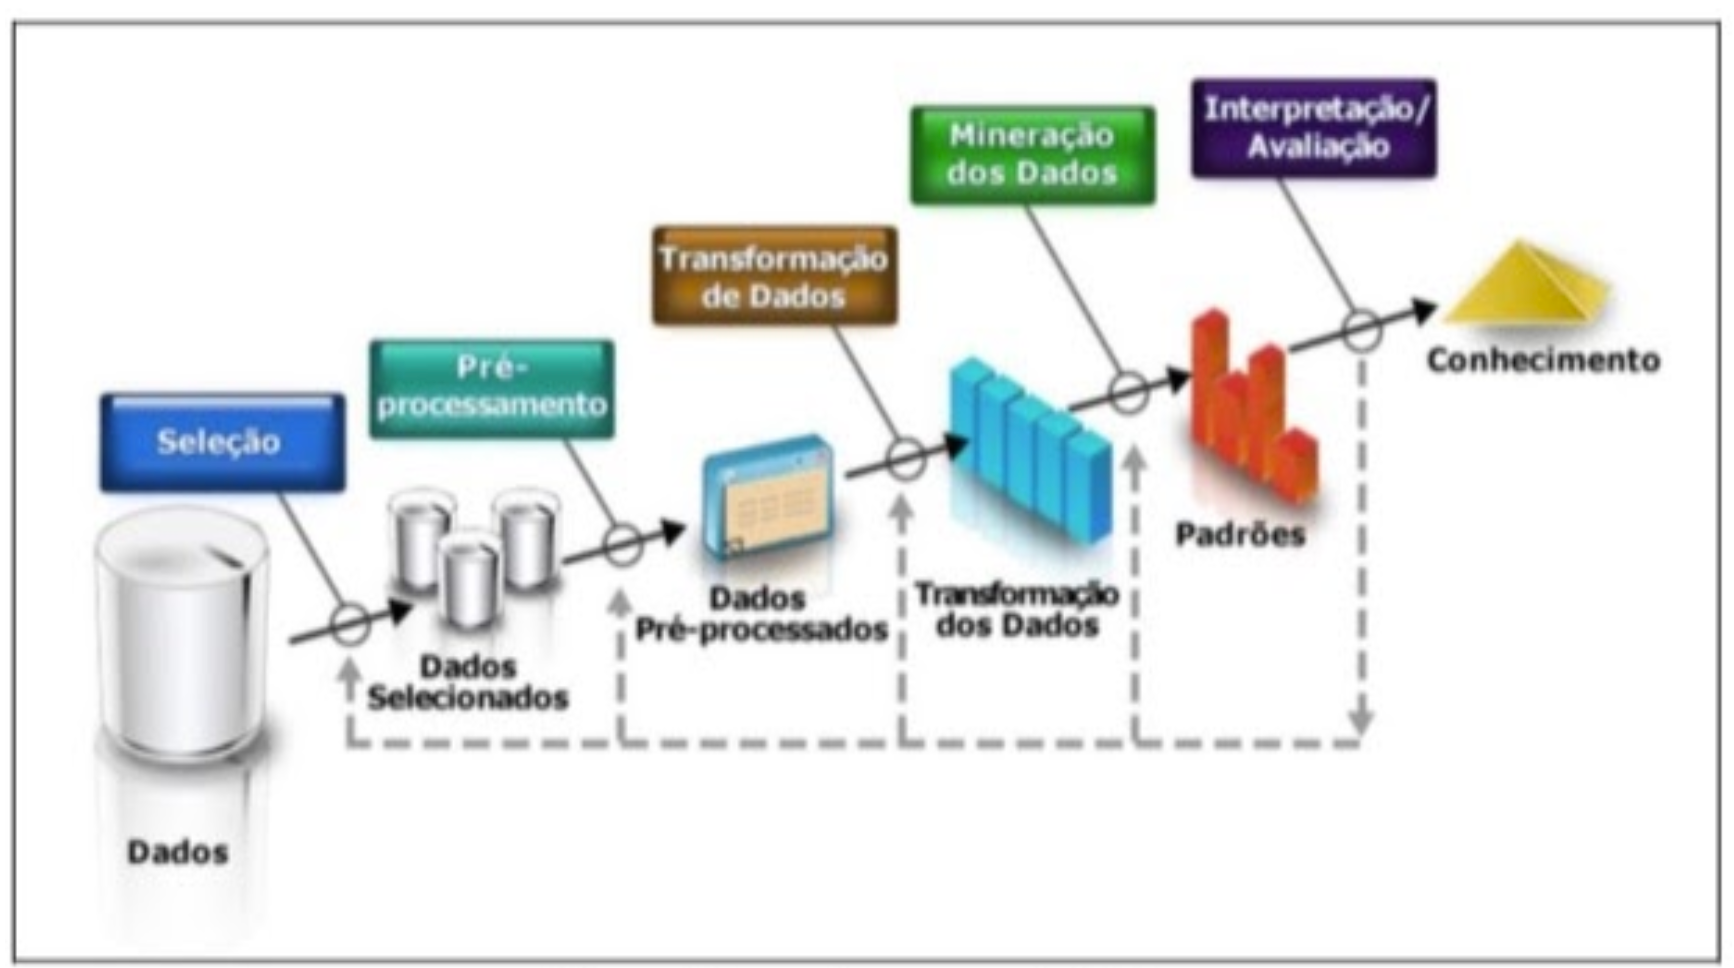
\includegraphics[width=0.6\textwidth]{./04-figuras/figura-11}
    \label{fig:ilustfig11}
\end{figure}
\vspace*{-0,9cm}
{\raggedright \fonte{adaptado de Fayyad et al (1996)}} \\

Suas características s\~{a}o:

\begin{itemize}

    \item Não trivial já que alguma técnica de busca ou inferência \'{e}envolvida (não \'{e}apenas um processo de computação direta);
    
    \item Os padrões descobertos devem ser válidos com algum grau de certeza, novos, trazer algum benefício e serem compreensíveis (se não imediatamente então depois da interpreta\c{c}\~{a}o.

\end{itemize}

Em nosso trabalho n\~{a}o iremos objetivar o uso dessa tecnologia, pois, n\~{a}o \'{e} a nosso inten\c{c}\~{a}o, mas, foi preciso informar da sua existência nesse tópico para que haja um aprofundamento teórico de tudo que envolve o mundo do BI. 

O processo \'{e} iterativo e, embora apresente uma defini\c{c}\~{a}o semelhante tamb\'{e}m ao minera\c{c}\~{a}o de dados, deve ser composto de uma s\'{e}rie de etapas sequenciais, podendo haver retorno a etapas anteriores, isto \'{e}, as descobertas realizadas (ou a falta delas). Eventualmente, este processo conduz a novas hipóteses e descobertas. Neste caso, o usu\'{a}rio pode decidir pela retomada dos processos de minera\c{c}\~{a}o, ou uma nova sele\c{c}\~{a}o de atributos, por exemplo, para validar as hipóteses que surgiram ao longo do processo.

O produto esperado da extra\c{c}\~{a}o de conhecimento \'{e} uma informa\c{c}\~{a}o relevante para ser utilizada pelos tomadores de decis\~{a}o. Alguns autores, por\'{e}m, defendem o ponto de vista de que o conhecimento descoberto n\~{a}o precisa necessariamente ser incorporado a um sistema de apoio \`{a} decis\~{a}o (SAD).

\section{OLAP (Processamento Analítico On-line)}

O OLAP \'{e}composto por inúmeras técnicas e ferramentas que possibilitam a exploração de dados armazenados em um data warehouse, utilizando técnicas que permitem a visualização de vários dados. Diariamente as organizações acumulam grandes quantidades de dados e o OLAP as ajuda a fazer uma análise mais segura e confiável desse grande volume de dados transformando-os em informações. (JACOBSON; MISNER, 2007).

O OLAP \'{e}composto por vários processos usados para criar, gerenciar e manipular os dados contido no banco de dados, o mesmo tem a função de agilizar a recuperação dos dados, podendo ainda executar e examinar uma grande quantidade de dados. Os gestores das empresas usam OLAP em qualquer setor da organização, pois lhes proporciona realizar análises comparativas para auxiliá-los nas decisões tomadas no dia-a-dia. (JACOBSON; MISNER, 2007).

Os sistemas OLAP são conhecidos por representar algumas características com:

\begin{itemize}
    
    \item Oferece aos usuários uma resposta às suas consultas com mais rapidez. Apresenta relatórios que antes eram difíceis de analisar devida sua complexidade de uma forma mais fácil, simples de entender.
    
    \item O OLAP oferece ferramentas para que os usuários possam criar seus próprios relatórios, com isso poderá analisar como anda o desenvolvimento das empresas de uma forma mais rápida e flexível; (LARSON; AGARWAL, 2006)
    Oferece uma forma interativa com o usuário durante a disponibilização das informações;
    
    \item Permite que haja uma repetição de dados para melhorar as consultas;
    Permite que se façam cálculos com uma complexidade alta e uma visualização desses cálculos em diversas dimensões; e;
    
    \item Permite que se façam ajustes para que as consultas se tornem mais segura, para que a partir desses resultados se possam concluir analises de tendências.

\end{itemize}

Uma organiza\c{c}\~{a}o, seja pública ou privada que usa OLAP terá um desempenho melhor diante das concorrentes, pois com o uso dessa técnica pode trazer informações com mais rapidez, da melhor forma para seu entendimento e tudo de uma forma bem interativa. 

Hoje no ambiente competitivo globalizado o que vale \'{e}ter informação e estar sempre informado do que esta acontecendo no mundo, mas, principalmente, dentro de sua própria empresa e essa técnica possibilita que todos os membros fiquem integrados do que acontece na organização de forma simples, rápida e interativa. (JACOBSON; MISNER, 2007).

Segundo KIMBALL (2002) o mesmo, classifica os sistemas OLAP em ROLAP, MOLAP, HOLAP E DOLAP, essas ferramentas possibilitam diferentes formas de organizar os dados antes de apresentá-los ao usuário final.

A ROLAP \'{e}utilizada nas análises mais exploratórias dos dados, sendo bastante utilizada pela área de marketing. 

Quanto à ferramenta MOLAP, permite análises mais simples e rápidas, mas, também, apresenta limitação de tamanho, tendo estrutura similar ao de uma planilha, com linhas e colunas. (MICROSOFT CORPORATION, 2007).

A HOLAP \'{e}o resultado da combinação entre as ferramentas MOLAP e ROLAP, extraindo o que há de melhor das duas. (MICROSOFT CORPORATION, 2007).

As ferramentas DOLAP \textit{(Desktop Online Analytical Processing)} disparam uma instrução
SQL \textit{(Structure Query Language)} de computador simples, configurado como cliente, com um servidor de dados que retorna um microcubo de informações a serem analisadas no cliente, permitindo o processamento da máquina cliente, sem problemas de tráfego de rede e nem problemas de escalabilidade. 

Porém existe uma desvantagem neste processo, o microcubo não deve ser muito grande para que não haja uma perda de largura de banda. (MICROSOFT CORPORATION, 2007)

\subsection{Tipos de opera\c{c}\~{a}o sobre OLAP}

Segundo BALLARD (2006), as principais operações utilizadas nas ferramentas OLAP são : \textit{Drill Across, Drill Down, Drill Up, Drill Throught, Alertas, Ranking, Filtros, Sorts, Breaks, Slice and Dice e o pivot.}

\begin{itemize}

    \item \textit{Drill Across}: ocorre quando o usuário atravessa um nível intermediário numa mesma dimensão. Ex: Ele executa um Drill Across quando há uma alteração de ano para mês diretamente;

    \item \textit{Drill Down}: ocorre quando o nível de detalhes da informação sofre um aumento;
    
    \\item textit{Drill Up}: ocorre quando o usuário diminui o nível de detalhes da informação, \'{e}o contrario do Drill Down;
    
    \item \textit{Drill Throught}: ocorre quando o usuário muda a informação de dimensão. Ex: Estás na dimensão tempo e no próximo passo estás analisando a informação por região (outra dimensão);
    
    \item Alertas: servem para informar sobre as situações importantes e mostrar os valores mediante as condições;
    
    \item \textit{Ranking}: possibilita juntar todos os resultados por ordem decrescente ou crescente, baseando-se em objetos numéricos conhecidos como as Measures;
    Filtros: d\~{a}o as permissões para os usuários aperfeiçoarem, as pesquisas (Query) solicitadas por mais de uma vez, como se fossem filtros de informações;
    
    \item \textit{Sorts}: serve para ordenar as informações de forma crescente ou decrescente, de acordo com a escolha do usuário;
    
    \item \textit{Breaks}: serve para agrupar as informações em blocos. Ex: O usuário que ver as informações por cidades, então ele executou um break. Após esta ação ter sido executada, as informações estarão agrupadas por cidades;
    
    \item \textit{Slice and Dice}: como o OLAP gera ou recupera um micro-cubo, o Slice and Dice têm a responsabilidade de fazer alteração na posição de uma informação, alterar linhas e colunas para facilitar a compreensão dos usuários e girar o cubo sempre que tiver necessidade, esse recurso faz parte das principais características da ferramenta;
    
    \item \textit{Pivot}: Permite a troca de linhas por colunas em uma tabela ou modificação da posição das dimensões em um gráfico. Ou seja, \'{e} o ângulo pelo qual os dados são visualizados.
    
\end{itemize}

Conforme KIMBALL (2002), o OLAP \'{e}uma tecnologia de banco de dados que foi otimizada para consulta e relatório, em vez de processamento de transações. Os dados de origem do OLAP são bancos de dado OLTP\textit{(Online Transactional Processing)} que são comumente armazenados em um \textit{Data Warehouse}.

Os dados OLAP são originados a partir desses dados históricos, e integrados em estruturas que permitem análise sofisticada, sendo organizados hierarquicamente e armazenados em cubos em vez de tabelas. Esta tecnologia \'{e}organiza de forma fácil as estruturas multidimensionais para agilizar o acesso aos dados a serem analisados. 

Logo, s\~{a}o a base dos relatórios de tabelas ou gráficos dinâmicos, e a exibição de resumos de alto nível, bem como a exibição de resultados detalhistas.

\subsection{Os componentes do OLAP}

Os tipos de dados que constituem os bancos de dados OLAP são as medidas e as dimensões, sendo as medidas, os dados numéricos, ou seja, as quantidades e médias que você usa para tomar decisões comerciais, e as dimensões s\~{a}o as categorias que você usa para organizar essas medidas.

Os bancos de dados OLAP auxiliam na organização dos dados por muitos níveis de detalhe, utilizando algumas categorias que serão descritas a seguir: (MICROSOFT CORPORATION, 2007).

\begin{itemize}

    \item Cubo: são formas de dados que ajudam na realização de análises, sem eles não seria possível realizar análises de dados em diversas dimensões. Eles possibilitam combinar o tempo, a geografia e os produtos com números de vendas de forma r\'{a}pida, eficiente e resumida, mais detalhes sobre cubo no tópico 2.9;
    
    \item Medida: são todos os valores numéricos encontrados na região central de um cubo, como por exemplo, as vendas, os lucros, as receitas e os custos, todos processados, agregados e analisados;
    
    \item Membro: \'{e} caracterizado por objetos que podem desempenhar um ou mais impacto de dados em uma hierarquia;
    Membro calculado: o valor de um membro \'{e}calculado enquanto esta ocorrendo uma execução por meio de uma expressão. O valor de um membro calculado pode ser originado do valor de outro membro;
    
    \item Dimensão: \'{e} composta por uma ou mais hierarquias organizadas de níveis em um cubo de uma forma que o usuário possa entender e assim usá-las para fazer análise de dados;
    
    \item Hierarquia: \'{e}uma forma de ordenação em diferentes níveis organizando os membros de uma dimensão de forma que cada membro tenha um possa ter um membro pai e zero ou at\'{e}mais membros filho. De acordo com a hierarquia o membro filho \'{e}inferior ao membro atual, já o pai está em um nível superior relacionado diretamente ao membro atual. O valor pai \'{e}no gera consolidado aos valores de todos os seus filhos;
    
    \item Nível: em um processo hierárquico, os dados podem ser ordenados em níveis de detalhe inferiores e superiores, como por exemplo, Ano, Semestre, Trimestre, Mês e Dia em uma hierarquia Tempo.

\end{itemize}

\subsection{As Aplica\c{c}ões do OLAP}

O OLAP \'{e}caracterizado por ser diversificado, podendo ser aplicado em diversos setores de uma organização como no setor de: (MICROSOFT CORPORATION, 2007)

\begin{itemize}

    \item Nas finanças: nesse setor com o uso de OLAP poderá ser realizada uma analise de balanço geral da empresa, fazer um orçamento, fluxo de caixa da empresa, contas à receber;
    \item Nas vendas: pode ser feita uma análise das vendas escolhendo a região, os produtos que mais foram vendidos nesta região, o vendedor responsável pelas vendas, entre outros dados;
    \item No Marketing : o OLAP possibilita que faça uma análise de mercados, lucratividade de produto, e fazer uma análise de preço ou volume;
    \item Nos Recursos Humanos: com os sistemas OLAP poderá ser feito uma análise de benefícios, fazer projeção de salários e analise de números de funcionários da empresa ou do setor; e;
    \item Na Manufatura: através dessa ferramenta OLAP pode-se gerenciar o estoque da empresa, os fornecedores, fazer planejamento de que produtos estão em demanda, analisar os custos dos materiais para fabricação dos produtos.

\end{itemize}

\subsection{As Ferramentas OLAP}

Os gestores das organizações tem a necessidade de uma ferramenta que os auxiliem na exploração dos dados que forneça informações confiáveis, que de acordo com a análise das mesmas possam os auxiliar na tomada de decisão. Para isso existem algumas ferramentas que poderão ajuda-los nesse processo de exploração e analise dos dados como o \textit{Mondrian} ou textit{Schema Workbench} , que ser\'{a} tema de um tópico especifico, e que faz parte do Pentaho.

\section{Cubo}

Segundo Carlo Vercellis (VERCELLIS, 2009), o projeto de DW e data mart são baseados em um paradigma multidimensional para a representação de dados que fornece grandes vantagens no momento da consulta de dados, ele pode garantir tempo de resposta rápida, mesmo em complexas consultas, enquanto no lado lógico, as dimensões naturalmente correspondem a critérios normais e facilmente entendíveis a usuários para realizarem suas análises.

A representação multidimensional \'{e}baseada em um esquema em estrela que contém os dois tipos de tabelas de dados, as dimensões e Fatos.
Com isso pode-se dizer que um cubo, \'{e}a estrutura multidimensional de dados que expressa a forma na qual os tipos de informações se relacionam entre si. \'{e}formado pela tabela Fato e pelas tabelas de dimensão que a circundam e representam possíveis formas de visualizar e consultar os dados (VERCELLIS, 2009).

Pode-se citar um exemplo de um cubo através de um conjunto de lojas, considerando o faturamento de um produto em um mês do ano, em uma loja. Na existência de um cubo tridimensional, uma dimensão representa os produtos, a outra o período e outra as lojas. A figura 12,  representa o exemplo.

% figuras
\begin{figure}[H]
	\vspace*{0,2cm}
    \centering
    \caption{Cubo}
    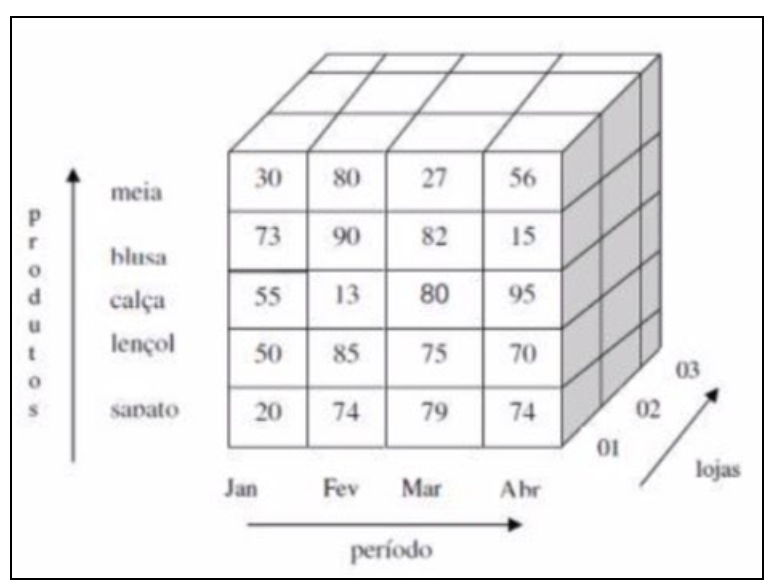
\includegraphics[width=0.6\textwidth]{./04-figuras/figura-12}
    \label{fig:ilustfig12}
\end{figure}
\vspace*{-0,9cm}
{\raggedright \fonte{VERCELLIS (2009)}} \\

\section{\textit{Data mining} (minera\c{c}\~{a}o de dados)}

Alguns profissionais da área de análise de informação enfrentam problemas no processo de transformar dados que as empresas acumulam em suas transações diárias em informações que serão de grande utilidade para o desempenho dos negócios. 

Assim, Segundo CORTES, o \textit{Data Mining} \'{e}um processo feito sobre enormes repositórios de dados como o \textit{data warehouse} buscando identificar padrões e alguma relação de consumo que não são conhecidos pela empresa e que podem ser usados na tomada de decisão. (CÔRTES, 2008).

Usando o \textit{Data Mining} esse problema será resolvido, pois ele \'{e}um processo pelo qual se descobri informações importantes para a empresa, como os padrões, as associações entre as informações da base de dados, mudanças, anomalias e as estruturas, em grandes quantidades de dados que são armazenados em base de dados ou outros repositórios de dados. (CÔRTES, 2008)
